% Stanford University PhD thesis style -- modifications to the report style
% This is unofficial so you should always double check against the
% Registrar's office rules
% See http://library.stanford.edu/research/bibliography-management/latex-and-bibtex
%
% Example of use below
% See the suthesis-2e.sty file for documentation
%
\documentclass[12pt]{report}
\usepackage[online]{suthesis-2e}
\usepackage{dblfloatfix}
\usepackage{graphicx}
\usepackage{todonotes}
\usepackage{floatrow}
\usepackage{wrapfig}
\usepackage{rotating}
\usepackage{subfigure}
\usepackage{epigraph}

%% Styling
\usepackage[T1]{fontenc}
\usepackage{AlegreyaSans} %% Option 'black' gives heavier bold face
\usepackage{Alegreya} %% Option 'black' gives heavier bold face
\renewcommand*\oldstylenums[1]{{\AlegreyaOsF #1}}
\usepackage{parskip}
\usepackage[all]{nowidow}
\usepackage[font={sf,small},labelfont=bf]{caption}

\usepackage{titlesec, blindtext, color}
\definecolor{gray75}{gray}{0.75}
\newcommand{\hsp}{\hspace{20pt}}
\titleformat{\chapter}[hang]{\Huge\bfseries\sffamily}{\thechapter\hsp
\textcolor{gray75}{|}\hsp}{0pt}{\Huge\bfseries}
\titleformat*{\section}{\bfseries\Large\sffamily}
\titleformat*{\subsection}{\bfseries\large\sffamily}
\titleformat*{\subsubsection}{\bfseries\sffamily}

%% This turns references into clickable hyperlinks.
\PassOptionsToPackage{hyphens}{url}\usepackage[bookmarks,backref=true,linkcolor=blue]{hyperref} %,colorlinks
\hypersetup{
  pdfauthor = {},
  pdftitle = {},
  pdfsubject = {},
  pdfkeywords = {},
  colorlinks=false,
  linkcolor= blue,
  citecolor= blue,
  pageanchor=true,
  urlcolor = blue,
  plainpages = false,
  linktoc=all
}

\usepackage[square,numbers,sort]{natbib}

% each of the following has two versions
%   \crefname{environmentname}{singular}{plural}, to be used mid-sentence
%   \Crefname{environmentname}{singular}{plural}, to be used at the beginning of a sentence
\usepackage{cleveref}

\crefname{chapter}{Chapter}{Chapter}
\crefname{section}{\S}{\S}
\crefname{table}{Table}{Tables}
\Crefname{table}{Table}{Tables}
\crefname{figure}{Fig.}{Figs.}
\Crefname{figure}{Figure}{Figures}

\dept{Computer Science}

%%%%%%%%%%%%%%%%%%%%%%%%%%%%%%%%%%%%%%%%%%%%%%%%%%%%%%%%%%%%%%%%%%%%%
% make complete reference clickable
\newcommand{\figref}[1]{\hyperref[#1]{Fig.~\ref*{#1}}}
\newcommand{\secref}[1]{\hyperref[#1]{\S\ref*{#1}}}
\newcommand{\tabref}[1]{\hyperref[#1]{Table~\ref*{#1}}}
\newcommand{\defref}[1]{\hyperref[#1]{Definition~\ref*{#1}}}
\newcommand{\equref}[1]{\hyperref[#1]{Eq.~\ref*{#1}}}
\newcommand{\lstref}[1]{\hyperref[#1]{Listing~\ref*{#1}}}

\begin{document}
\title{The Reactive Vega Stack:\\Declarative Interaction Design\\for Data
Visualization}
\author{Arvind Satyanarayan}
\principaladviser{Jeffrey Heer}
\coprincipaladviser{Maneesh Agrawala}
\secondreader{James Landay}

\tablespagefalse

\beforepreface
% !TEX root = ./thesis.tex
\prefacesection{Abstract}

Interactive visualization is an increasingly popular medium for analysis and
communication as it allows readers to engage data in dialog. Hypotheses can be
rapidly generated and evaluated in situ, facilitating an accretive construction
of knowledge and serendipitous discovery. Crafting effective visualizations,
however, remains difficult. Programming toolkits are typically required for
custom visualization design, and impose a significant technical burden on users.
Moreover, existing models of visualization relegate interaction to a
second-class citizen: imperative event handling callbacks that are difficult to
specify, and even harder to reason about.

This thesis introduces the \emph{Reactive Vega stack}: two new declarative
languages that lower the threshold for authoring interactive visualizations, and
enable higher-level reasoning about the interaction design space. \emph{Reactive
Vega} is an expressive, low-level representation that is well-suited for custom,
explanatory visualizations. It shifts the burden of execution from the user to
the underlying streaming dataflow system. \emph{Vega-Lite} builds on Vega to
provide a higher-level grammar for rapidly specifying interactive graphics for
exploratory analysis. Its concise format decomposes interaction design into
semantic units that can be systematically enumerated.

Together, these languages serve as platforms for further research into novel
methods of expressing visualization design, and systems for interactive data
analysis. And, critically, they provide a growing and engaged community to study
their use with -- the Wikipedia and Jupyter communities, for instance, have
embraced Vega and Vega-Lite to author interactive visualizations within articles
and data science notebooks, respectively. This thesis explores this nascent
space of higher-level interactive data systems with \emph{Lyra}, an interactive
visualization design environment (VDE).
% !TEX root = ../thesis.tex
\prefacesection{Acknowledgments}
\label{sec:acknowledgements}

By every measure, Jeffrey Heer has been a consummate advisor. Early in my
graduate student career, I was confronted with a fork in the road: remain at
Stanford, a place I had worked hard to get to, or follow Jeff up to the
University of Washington. Though I had to leave behind a significant other and a
fledgling start-up, the choice was clear. It was Jeff's warmth, insight, and
vision that had attracted me to Stanford; if he was moving, so must I! This
dissertation more than validates that decision. Jeff has helped me not only grow
as a researcher but, by frequently diving deep into the Vega code base, hone my
software engineering skills as well. His commitment to producing high-caliber
research \emph{and} ensuring it is released as open-source work remains an
ongoing source of inspiration. If I am half the advisor he is, my future
students will be very luck indeed!

I have also been fortunate to have had the guidance of several other mentors. My
undergraduate advisor, Jim Hollan, fueled my interest in human-computer
interaction. A summer in his lab, where he gave me free reign to explore
questions in multimodal interaction, launched my research career and his
continued counsel to \emph{"never let the urgent drive out the important"} kept
me grounded. Wendy Mackay and Michel Beaudouin-Lafon have been critical for
understanding the broader implications of my work (and for giving me ample
excuses to visit Paris!). I am particularly excited about working with them on
some of the future research directions we brainstormed over drinks or in the
back of their car! Thank you also to Maneesh Agrawala, James Landay, Chris
R\'{e}, and Jeff Hancock for their time, generosity, and sage advice about the
academic job market.

I am also indebted to my incredible collaborators and colleagues at both
Stanford and the University of Washington. Little of the work described in this
thesis would have been possible without the talent and dedication of Kanit
Wongsuphasawat, Dominik Moritz, Jane Hoffswell, and Ryan Russell. The warm
welcome from Danielle Bragg, Caitlin Bonnar, Felicia Cordeiro, and Daniel
Epstein quickly made me feel like a member of the UW community. And, the
48-hour, caffeine-fueled, pre-CHI-deadline Webzeitgeist session with Ranjitha
Kumar, Jerry Talton, Maxine Lim, and Cesar Torres remains one of my favorite
graduate school memories. Thank you also to staff in both departments, including
Jillian Lentz, Jayanthi Subramanian, Monica Niemiec, Diane Rosano, and Andrea
Kuduk, for their patience with my uncountable administrative questions.

My work has been generously supported first by an SAP Stanford Graduate
Fellowship and later by a graduate fellowship from Google. I credit the
widespread adoption of the Reactive Vega stack, in part, to the opportunities we
have had to spread the word. To that end, I am grateful to our external
collaborators including Irene Ros, Lynn Cherny, K. Adam White, Sue Lockwood,
Jake Vanderplas, Brian Granger, and Yuri Astrakhan.

I am fortunate that graduate school has mostly offered me very high highs. But,
for the occasional low low, I am thankful to have been able to commiserate,
rant, and drink with a fantastic group of friends including Marianne Lontoc,
Patrick Mutchler, Rachel Midura, Lauren Howe, Ben Poole, Megan Lin, Austin
Gibbons, and Jessie Schroeder.

Finally, I dedicate this thesis to my family. To my parents, Manju and Satya,
for fostering my interest in computing, often ``forgetting'' I had used up my
alloted screen time for a particular day! Your unconditional love gave me the
support I needed to forge an identity and career half a world away. And to the
love of my life, Maeva Fincker, for being my rock these past four years. I am so
very lucky to have you on my team, to celebrate my successes, and to confide in
you my fears.

Thank you.
\afterpreface

% !TEX root = ./thesis.tex
\chapter{Introduction}

\vspace{-35pt}

\setlength\epigraphwidth{.75\textwidth}
\epigraph{\textit{A graphic is not ``drawn'' once and for all; it is
``constructed'' and reconstructed until it reveals all the relationships
 constituted by the interplay of the data. The best graphic operations are those
 carried out by the decision-maker himself.}} {\textit{Graphics and Graphic
 Information Processing}\\\textsc{Jacques Bertin, 1981}}

Data visualization has gone mainstream. From business intelligence to data
journalism, society has embraced visualization as a medium for recording,
analyzing, and communicating about data. This explosion of use is reflected in
the proliferation of visualization tools, which span the gamut of expressivity.
At one end are chart templates (e.g., Google Fusion Tables, or as found in
spreadsheet packages such as Microsoft Excel). Users can easily generate
recognizable output by choosing from a pre-defined palette of chart types, but
only a handful of properties may be customized. At the other end are vector
graphics programs (e.g., Adobe Illustrator), and low-level programming APIs
(e.g., Processing or OpenGL). Users have complete control but the added
expressivity trades-off ease-of-use.

Advances in visualization toolkits have popularized \emph{grammar-based}
approaches for visual encodings
\cite{wilkinson:grammar,stolte:polaris,wickham:layered,bostock:protovis,bostock:d3}.
These models are more expressive than chart templates as they decompose the
design space into combinatorial primitives for data transformation and visual
encoding. Moreover, they embody \emph{declarative design}\,---\,the languages
describe \emph{what} the visualization should look like, rather than \emph{how}
it should be rendered. As a result, users are free to focus on visual encoding
and design decisions while the underlying runtime is entirely responsible for
execution concerns and performance optimization~\cite{heer:protovisjava}.

However, key challenges remain. Interaction is critical for effective
visualization, allowing users to interrogate data and iteratively refine their
mental models~\cite{pike:interactionscience,yi:understanding}. Yet, existing
declarative visualization models provide poor support for interaction
techniques. Simple ``interaction typologies'' (e.g., brushing, panning, etc.)
are available, but limit customization. Thus, users often author
\emph{imperative} event handling callbacks that undo the benefits of declarative
design. Users are forced to manually maintain state~\cite{cooper:embedding} and
coordinate interleaved execution\,---\,a complex and error-prone task
colloquially called ``callback hell''~\cite{edwards:coherent}.

Moreover, most existing declarative models (including
ggplot2~\cite{wickham:layered} and D3~\cite{bostock:d3}) are instantiated via
complex APIs embedded in programming languages. This approach imposes a
non-trivial \emph{articulatory distance}~\cite{hutchins:directmanip} as users
must map their desired \emph{visual} output to \emph{textual} commands\,---\,a
fundamental mismatch in representations.

\vspace{-10pt}

\section{Thesis Contributions and Outline}

This dissertation is divided into seven chapters, and contributes a layered
stack of new declarative languages for \emph{interactive} visualization as well
as a new interactive system for visualization design through direct
manipulation.

\Cref{sec:related_work} surveys prior work that this dissertation builds on,
including a panoply of visualization toolkits and systems, methods from
functional programming languages and streaming database systems, and generative
models of user interfaces.

\Cref{sec:vg:lang} introduces Reactive Vega: a declarative language for
interactive data visualization that models user interaction as \emph{streaming
data}. Alongside established declarative visual encoding primitives, Reactive
Vega introduces event streams and signals, two constructs from Functional
Reactive Programming. Event streams, defined with a novel CSS-inspired selector
syntax, abstract the complexity of capturing and sequencing input events. Event
streams drive signals: dynamic expressions that are automatically reevaluated
when new events fire. Signals parameterize visual encoding primitives, thereby
endowing them with reactive semantics\,---\,when a new event fires, it is
propagated to corresponding signals; dependent visual encodings are reevaluated
and the visualization is automatically re-rendered. Additional primitives allow
interaction techniques to be generalized and reused across distinct
visualizations. This chapter demonstrates Reactive Vega's expressivity through
example visualizations that cover an established interaction taxonomy.

\Cref{sec:vg:arch} studies the implications of declarative interaction design on
the architecture of visualization systems. The Reactive Vega architecture adapts
and extends techniques from streaming database systems. In particular, an input
declarative specification (expressed as JavaScript Object Notation) is parsed to
construct a dataflow graph. Dataflow operators perform computations on
\emph{changesets} of tuples or scene graph elements, and are \emph{replayed} if
signal parameter values change. To support data-driven multi-view displays, the
dataflow graph is conditioned on data values. As new tuples are observed, or as
interaction events occur, the graph \emph{dynamically rewrites itself} at
runtime by extending or pruning branches. Performance optimizations are
described and comparative benchmark studies conducted to evaluate Reactive
Vega's performance. These studies find that Reactive Vega meets or exceeds the
performance of D3~\cite{bostock:d3} and the prior Vega system.

\Cref{sec:vega-lite} introduces Vega-Lite: a higher-level grammar that builds on
Reactive Vega. Vega-Lite extends a traditional grammar of graphics with a
\emph{view composition algebra} for layered and multi-view displays. A novel
\emph{grammar of interaction} features \emph{selections}: an abstraction that
encapsulates input event processing, points of interest, and a predicate
function for inclusion testing. Selections parameterize visual encodings by
serving as input data, defining scale extents, or by driving conditional logic.
Vega-Lite specifications are concise through ambiguity: lower-level details
(e.g., the events that trigger a selection) can be omitted and are filled in by
the Vega-Lite compiler. The smaller language surface area also facilitates
higher-level reasoning tasks, such as systematic enumeration of alternative
designs. These language properties are reified by recreating the examples from
\Cref{sec:vg:lang}.

\Cref{sec:lyra} introduces Lyra: an interactive environment that leverages both
Reactive Vega and Vega-Lite for visualization design by direct manipulation.
Through drag-and-drop interactions, users bind data values to mark properties.
Data transformations and layout algorithms are visually specified and inspected
with a ``data pipeline'' interface. As a higher-level graphical interface, Lyra
allows users to fluidly move between the different levels of abstraction. Direct
manipulation interactions generate statements in Vega-Lite, which are compiled,
and merged into a backing Reactive Vega specification; the visual inspectors
provide complete control over the latter. Thus, users can iterate between
rapidly creating recognizable output and making fine-grained
customizations\,---\,an approach that yields a diverse range of visualizations
without writing a single line of code.

Finally, \Cref{sec:conclusion} sketches new research directions that Reactive
Vega and Vega-Lite enable. These systems have been released as open-source
projects, and have already been used to power the Voyager visualization
recommendation browser~\cite{voyager,voyager2,compassql}, develop a model for
sequencing visualizations~\cite{kim:graphscape}, and reverse-engineer
visualizations from chart images~\cite{poco:reverse}. Moreover, the broader
adoption both tools have seen\,---\,Vega is used to embed interactive
visualizations within Wikipedia articles, and Vega-Lite can be used within
Jupyter notebooks\,---\,provide a growing, engaged user community to study their
use with.

\vspace{-20pt}

\section{Prior Publications and Authorship}

\vspace{-7pt}

Although I am the principal author for the research detailed in this
dissertation, it is also the product of several years of collaboration with my
primary advisor, Jeffrey Heer, and my colleagues at the University of Washington
Interactive Data Lab. The Reactive Vega language (\Cref{sec:vg:lang}) appeared
at \textsc{acm uist} 2014~\cite{satyanarayan:declarative} with Kanit
Wongsuphasawat contributing a prototype implementation of the reactive runtime.
The Reactive Vega architecture (\Cref{sec:vg:arch}) was published at
\textsc{ieee vis} 2015~\cite{reactive-vega-arch}, with Ryan Russell and Jane
Hoffswell contributing example visualizations and designing the figures.
Vega-Lite (\Cref{sec:vega-lite}) is joint work with Dominik Moritz and Kanit
Wongsuphasawat. It was published at \textsc{ieee vis} 2016~\cite{vega-lite} and
my co-authors led the design and implementation of the visual encodings.
Finally, Lyra was published at EuroVis 2014~\cite{lyra}. To reflect the
contributions of my collaborators, I will use the first-person plural (we) in
these chapters.
% !TEX root = ./thesis.tex
\chapter{Related Work}
\label{sec:related_work}

This dissertation builds on prior work in visualization systems, programming
languages, streaming databases, and human-computer interaction. In this chapter,
I survey pertinent work in each domain and describe how this thesis extends
them.

\section{Visualization Toolkits \& Systems}

Chart templates, as found in spreadsheets and online services (e.g., Many
Eyes~\cite{ibm:manyeyes} and Google Fusion Tables), are a common means for
creating visualizations: users select from a pre-defined palette of chart types.
Such \emph{chart typologies} are popular because they are simple to use and
efficient\,---\,users can produce a recognizable chart with only a few clicks.
This approach, however, is closed. Users are restricted to only the available
chart types, and may customize only a small handful of parameters.

To enable custom visualization design, researchers have developed programming
toolkits that offer a number of visualization components. For instance, the
InfoVis Toolkit~\cite{fekete:ivtk} provides a class hierarchy of visualization
widgets, where new visualizations are created by subclassing existing components
or writing new ones. In contrast, Prefuse~\cite{heer:prefuse} and
Flare~\cite{flare} offer composable operators for data transform, layout, and
encoding. While either approach offers fine-grained control over visual output,
they both constrain expressivity much like chart typologies. Novel designs
require new widgets or operators, and significant software engineering effort.

\subsection{Grammar-Based Visual Encoding}

In 1999, Leland Wilkinson introduced an alternative approach with \emph{The
Grammar of Graphics}~\cite{wilkinson:grammar}. Eschewing chart typologies in
favor of a combinatorial building blocks, Wilkinson's grammar yields a more
expressive design space and allows users to rapidly construct visualizations.
Provided abstractions include primitives for data modeling and transformation,
visual encodings defined as mappings between data fields and channels (e.g.,
position, color, and size), and scales and guides (i.e., axes and legends). His
work was quickly followed by the Stanford Polaris system~\cite{stolte:polaris}
(commercialized as Tableau), and Hadley Wickham's popular
ggplot2~\cite{wickham:layered} package implements a variant of this model in the
R statistical language.

These tools focus on statistical graphics for exploratory analysis and, to that
end, favor concise specification languages. Analysts may omit details such as
scale transforms (e.g., linear or log) or color palettes, which are then filled
in by the grammar using a rule-based system of smart defaults. As a result,
analysts are able to rapidly generate visualizations, analyze them, and continue
with their analysis process.

Through the lower-level Protovis~\cite{bostock:protovis,heer:protovisjava} and
D3~\cite{bostock:d3} languages, Bostock and Heer describe how a similar approach
can enable expressive design for custom, explanatory graphics as well. Perhaps
most importantly, they articulate the advantages of declarative design for data
visualizations: by separating specification from execution, declarative
languages facilitate an iterative development process, can transparently
optimize processing, and simplify retargeting across
platforms~\cite{heer:protovisjava}.

The design of Reactive Vega and Vega-Lite is heavily influenced by these works.
Reactive Vega's visual encoding primitives and implementation pipeline closely
mirror Protovis'. Marks including \emph{arcs}, \emph{areas}, \emph{bars},
\emph{lines}, plotting \emph{symbols} and \emph{text} are processed through
\emph{bind}, \emph{build}, and \emph{evaluate} stages to generate a scene graph.
Protovis' \emph{panel} marks are renamed to \emph{group} marks, and enable the
repeated and nested structures found in small multiple displays. Marks can be
positioned relative to one-another with Vega's \emph{reactive geometry}, which
provides a more unified approach to layout as compared with Protovis'
\emph{anchors}.

Similarly, Vega-Lite represents basic plots using a set of encoding definitions
that map data attributes to visual channels, and may include common data
transformations. Vega-Lite differs most from other high-level grammars in its
approach to multiple view displays. Each of these grammars supports faceting (or
nesting) to construct trellis plots in which each cell similarly visualizes a
different partition of the data. Both Wilkinson's grammar and Polaris/Tableau
achieve this through a \emph{table algebra} over data fields, which in turn
determines spatial subdivisions. Tableau additionally supports the construction
of multi-view dashboards via a different mechanism, with each view backed by a
separate specification. In contrast, Vega-Lite contributes a \emph{view
algebra}: starting with unit specifications that define a single plot, Vega-Lite
expresses composite views using operators for layering, horizontal or vertical
concatenation, faceting, and parameterized repetition. When applicable, these
operators will merge scale domains and properly align constituent views.
Disparate views can also be combined into arbitrary dashboards, all within a
unified algebraic model.

\subsection{Dataflow Visualization Systems}

Dataflow architectures are common in scientific visualization systems, such as
IBM Data Explorer~\cite{lucas:dataflow,abram:ibmdx} and
VTK~\cite{schroeder:vtk}. Developers must manually specify and connect each
required operator into a network, which can support updates in a demand-driven
fashion (e.g., as data is modified) or an event-driven fashion (e.g., in
response to user input). These systems expose fine-grained control over the
construction of the dataflow graph. For example, VTK developers can choose to
favor memory efficiency over processing speed, which causes dataflow operators
to delete their output after computation. While Reactive Vega shares some
dataflow strategies with these systems\,---\,for example, using
pass-by-reference for unchanged tuples to reduce memory consumption\,---\,it
abstracts such execution concerns away from the user. The dataflow graph is
automatically assembled based on definitions found in a declarative
specification, and optimizations are transparently performed such that output
data is only stored when needed by downstream operators and shared otherwise.

Within the domain of information visualization, the Stencil
language~\cite{cottam:stencil} is also grounded in reactive semantics and uses a
dataflow model. Like Reactive Vega, it provides a unified data model where both
input data and interaction events are modeled as first-class streaming data
sources. However, Reactive Vega is more expressive than Stencil in two important
ways. First, Stencil does not provide primitives, beyond event streams, to
support interaction design; Reactive Vega, on the other hand, offers predicates
and scale inversions to lift interactive selections into data queries, and
coordinate multiple displays. Moreover, graphical primitives can be arbitrarily
nested with Reactive Vega, drawing from either hierarchical or distinct data
sources. This ability is critical to concisely specifying small multiples
displays, and requires Reactive Vega's dataflow graph to dynamically rewrite
itself at runtime. To the best of our knowledge, Stencil's architecture does not
support self-instantiating dataflows.

Improvise~\cite{weaver:improvise} features active variables called ``live
properties,'' which provide a basic form of reactivity\,---\,they may be bound
to control widgets and parameterize a visualization. Using an expression
language, live properties are assembled into a coordination graph to dynamically
evaluate visual encodings and generate views of data. While Improvise and
Reactive Vega share some conceptual underpinnings, Improvise places a higher
burden on users to correctly construct the necessary graph. As Reactive Vega
takes a declarative approach to visualization design, users need only compose
the necessary primitives into a specification. Reactive Vega parses this
specification to build the corresponding dataflow graph.

\subsection{Interactive Visualization Systems}

Besides text-based toolkits, researchers have also developed graphical user
interfaces for constructing visualizations.
Polaris/Tableau~\cite{stolte:polaris}, for instance, displays a ``schema'' panel
that lists available data fields. Data groupings and visual encodings are
specified by dragging these fields onto ``shelves'' that array the periphery of
the visualization. Lyra extends this mode of interaction onto the visualization
canvas itself\,---\,property \emph{drop zones} overlay marks during drag
operations, providing a more direct data-mapping target.

Roth et al.'s SageBrush~\cite{roth:sagebrush} supports similar interactions.
Users can drag-and-drop ``partial prototypes'' for spatial encodings and
``grapheme'' (mark) primitives such as lines and bars. Custom grapheme
properties are manually selected via menus, then exposed as drop-target icons.
Lyra refines the SageBrush model in several ways. Partial prototypes in
SageBrush implicitly define scale transforms and layout; by leveraging the Vega
and Vega-Lite grammars, Lyra decouples these components to support richer
designs. Lyra's data pipelines provide an extensible set of data
transformations, and different marks can be driven by unique pipelines and
composed. Finally, Lyra eschews iconic abstractions in favor of direct drop
zones for mark properties, without need of explicit enumeration via menus.

More recently, Bret Victor demonstrated a data-driven drawing
tool~\cite{victor:drawing} (now developed as
Apparatus\footnote{http://aprt.us/}) that combines geometric constraints with
\emph{imperative} procedures over data. Alongside an interactive canvas and data
table viewer, the tool includes programming structures with lexical scope and
control flow via loops and conditionals. To form a basic bar chart, designers
must define loops to create and position each bar. The tool supports purely
geometric constructions, rendering some layouts inexpressible. By building on
Vega and Vega-Lite, Lyra takes a \emph{declarative} approach to design. When a
designer associates a mark with a dataset, one mark instance per datum is
automatically produced rather than requiring explicitly instantiation by the
designer. More advanced algorithms, which are difficult to express with Victor's
tool, are accessible as part of Lyra's graphical data pipeline.

\section{Specifying Interactions in Visualizations}

Despite the central role of interaction in effective data visualization
\cite{heer:dynamics, pike:interactionscience}, little work has been done to
develop a grammar for specifying interaction techniques. Wilkinson's grammar
includes no notion of interaction. Tableau supports common interaction
techniques, but relies on mechanisms external to the visual encoding grammar.
Early systems like GGobi~\cite{swayne:ggobi} support common techniques as well,
and provide imperative APIs for custom methods. However, such APIs make easy
tasks needlessly complex, burdening developers with learning low-level execution
details. More recent systems, including Protovis, D3, and
VisDock~\cite{choi:visdock}, offer a typology of common techniques that can be
applied to a visualization. Such top-down approaches, however, limit
customization and composition. For example, D3's interactors encapsulate event
processing, making it difficult to combine them if their events conflict (e.g.,
if dragging triggers brushing \emph{and} panning).

\subsection{Interactive Selection \& Querying}

Selection, often in the form of users clicking or lassoing visual items, is a
fundamental operation in user interfaces and has been well-studied in the
context of data visualization. For example, in Snap-Together
Visualization~\cite{north:snap}, multiple views are coordinated via ``primary-''
and ``foreign-key actions,'' which propagate selected data tuples from one view
to the others. Wilhelm~\cite{wilhelm:interaction} describes the need for such
``indirect object manipulation'' methods as an axiom of interactive data
displays. Chen's compound brushing~\cite{chen:compound} provides a visual
dataflow language for specifying a rich space of transformations of brush
selections.  More recently, Brunel~\cite{brunel} provides a special
\texttt{\#selection} data field that is dynamically populated with the elements
a user interacts with, and can be used to link multiple views or filter input
data. Similarly, RStudio's Shiny~\cite{shiny}, an imperative web application
layer, provides \texttt{brushedPoints} and \texttt{nearestPoints} functions
which can be used to operate on selected elements.

Other systems have studied formally representing selections as data
queries~\cite{wilhelm:interaction}. For example, brushing interactions in
VQE~\cite{derthick:interactive} generate \emph{extensional} queries that
enumerate all items of interest; a form-based interface enables specification of
\emph{intensional} (declarative) queries. Individual point and brush selections
in DEVise~\cite{livny:devise}, known as \emph{visual queries}, map to a
declarative structure and are used to link together multiple views. With
VIQING~\cite{olsten:viqing}, rectangular ``rubber band'' selections are modeled
as range extents, and views can be dropped on top of each other to join their
underlying datasets. Heer et al.~\cite{heer:generalized} demonstrate that by
modeling a selection as a declarative query, interactive ``query relaxation''
can successively capture more items of interest.

Reactive Vega and Vega-Lite both build on this work with abstractions for
constructing selections. In Reactive Vega, \emph{predicates} express interactive
selections in visual space, are lifted to data queries by inverting them through
scale functions, and participate in if-then-else chains to manipulate visual
encoding rules. Vega-Lite abstracts these primitives with a higher-level
\emph{selection}. Vega-Lite selections are populated with one or more points of
interest, in response to user interaction. Their built-in predicates map to
declarative queries, thereby allowing a minimal set of ``backing'' points to
represent the full space of selected points. Additional operators can transform
a selection's predicate or backing points (e.g., offsetting them to translate a
brush selection or perform panning). Selections parameterize visual encodings by
driving conditional logic, serving as input data, or defining scale extents.

\section{Alternate Paradigms for Imperative Callbacks}

For custom interaction design with existing visualization toolkits, users must
author imperative event handling callbacks which present several development
hurdles~\cite{myers:callbacks}. Callbacks registered outside the visualization
specification allow users to externally manipulate visualization state and
manually update dependencies~\cite{cooper:embedding}. This approach breaks
encapsulation and necessitates the introduction of side-effects: external calls
to maintain state~\cite{cooper:integrating}. Callback execution order can also
be unpredictable, requiring users to coordinate interleaved
calls~\cite{edwards:coherent}. As a result, callbacks can make it difficult to
reason about the current state of the visualization, which is now the product of
both the original specification and the side-effects of interaction callbacks.

\subsection{Constraint Programming}

One alternative to callback-oriented imperative programming is constraint-based
specification. Systems like Gilt~\cite{myers:callbacks} and
$\mu$constraints~\cite{hudson:constraints} implement one-way constraints: when
the value of a constrained interface is modified, its dependents are
automatically affected. Other systems, like Cassowary~\cite{badros:cassowary},
implement two-way constraints using more complex constraint solvers. Recently,
ConstraintJS~\cite{oney:constraintjs} and Bret Victor's prototype for drawing
data visualizations~\cite{victor:drawing} have shown that constraint programming
is suitable for authoring web applications and data visualizations,
respectively.

However, while constraint systems remove many of the obstacles introduced by
callbacks, they do not involve general consideration of event handling\,---\,a
crucial element for interaction design. In fact, the authors of ConstraintJS
intend for their system to complement event
architectures~\cite{oney:constraintjs}.

\subsection{Functional Reactive Programming}

Functional Reactive Programming (FRP) formalizes semantics similar to one-way
constraints. Drawing from dataflow programming, FRP recasts mutable values as
continuous, time-varying data streams~\cite{bainomugisha:frpsurvey}. We focus on
a discrete variant called Event-Driven FRP (E-FRP)~\cite{wan:efrp}. To capture
value changes as they occur, E-FRP provides \emph{streams}, which are infinite
time-ordered sequences of discrete events. Streams can be composed into
\emph{signals} to build expressions that react to events. The E-FRP runtime
constructs the necessary dataflow graph such that, when a new event fires, it
propagates to corresponding streams. Dependent signals are evaluated in a
two\--phase update: in the first phase, signals use prior computed values of
their dependents, which are subsequently updated in the second phase. E-FRP has
been shown to be viable for authoring interactive web
applications~\cite{czaplicki:elm, meyerovich:flapjax} and
visualizations~\cite{cottam:stencil, kelleher:modeljs}.

Reactive Vega's declarative interaction primitives remain grounded in E-FRP
semantics, and they preserve the two-phase update: interdependent signals are
updated in the order in which they are defined in the specification. However,
naive applications of E-FRP to visualization tasks can result in wasteful
recomputation. Traditional E-FRP primitives support only \emph{scalar} values,
whereas visualization pipelines must also process relational and hierarchical
data. Modeling these latter data types as scalar values provides insufficient
granularity to perform targeted recomputation. To efficiently support relational
data, Reactive Vega integrates streaming database methods; and, to support
streaming hierarchical data, the dataflow graph dynamically rewrites itself at
runtime, instantiating new branches to process nested relations.

\section{Data Stream Management}

The problem of managing streaming data has been well studied in the database
community. Researchers have developed an arsenal of techniques through the
development of systems such as Aurora~\cite{abadi:aurora},
Eddies~\cite{avnur:eddies}, STREAM~\cite{arasu:stream}, and
TelegraphCQ~\cite{chandrasekaran:telegraphcq}. As tuples are observed by these
systems, they are flagged as either new or removed. Tuples, rather than full
relations, are passed between operators in a query plan (realized as a dataflow
graph). As a result, operators can inspect just the updated tuples to perform
efficient computation. However, for some operations a set of changed tuples is
insufficient. For example, a join of two relations requires access to all tuples
within a specified window. In such cases, caches (sometimes referred to as
\emph{views}~\cite{abadi:aurora} or \emph{synopses}~\cite{arasu:stream}) are
used to materialize a relation, and shared among dependent operators.

Borealis~\cite{abadi:borealis} extends this work in two ways. To support
streaming tuple modifications, it introduces a revision processing scheme. An
operator can be \emph{replayed} with revised tuples in place of the original
data, and will then only emit corresponding revisions. Similarly, to enable
dynamic operator parameters, Borealis introduces \emph{time travel}. When an
operator parameter changes, an \texttt{undo} is issued to the nearest cache. The
cache emits tuple deletions, effectively ``rewinding'' the system to a previous
time. A subsequent \texttt{replay} triggers recomputation with the new parameter
value.

However, existing streaming data systems concern flat relations. Reactive Vega
instantiates these techniques, alongside E-FRP, within a visualization pipeline
and extends them to support streaming nested data. To do so, Reactive Vega's
dataflow graph dynamically rewrites itself at runtime with new branches. These
branches unpack nested relations, enabling downstream operators to remain
agnostic to higher-level structure while supporting arbitrary levels of nesting.

\section{Generative Models of User Interfaces}

Michel Beaudoin-Lafon's instrumental interaction
paradigm~\cite{beaudouin:instrumental} helped motivate this dissertation's
approach of considering declarative interaction design at varying levels of
abstraction. He identifies three properties of interaction models for post-WIMP
interaction: \emph{descriptive} of existing and new techniques;
\emph{comparative} to evaluate alternative designs; and, \emph{generative}, to
facilitate the identification and creation of new points in the design space.
Reactive Vega only offers the first property\,---\,an expressive design
space\,---\,but is too low-level to be generative or facilitate evaluation of
similar behaviors. Vega-Lite, on the other hand, offers both an expressive and
generative design space, suitable for exploring alternative techniques as
demonstrated in~\Cref{sec:vl:examples}. Kim et al. also demonstrate its
comparative powers, using Vega-Lite to model optimal sequences of
visualizations~\cite{kim:graphscape}.

Moreover, our articulation of Vega-Lite as a parametric design language is
inspired by Mackinlay's APT~\cite{mackinlay:apt} and his follow-on work with
Card and Robertson conducting a morphological analysis of input
devices~\cite{card:morphological}. In particular, we sought to identify and
decouple orthogonal axes of the design space. While \Cref{sec:vl:examples}
begins to systematically consider points along these axes, a full morphological
analysis of the Vega-Lite design space is left to future work.
% !TEX root = ./thesis.tex
\graphicspath{{./vega-lang/figures/}}
\chapter{Declarative Primitives for Interaction Design}
\label{sec:vg:lang}

Reactive Vega builds on a long-running thread of research on declarative
visualization design, popularized by the Grammar of
Graphics~\cite{wilkinson:grammar} and Polaris~\cite{stolte:polaris} (now
Tableau).

Visual encodings are defined by composing graphical primitives called
\emph{marks}~\cite{bostock:protovis}, which include \emph{arcs}, \emph{areas},
\emph{bars}, \emph{lines}, plotting \emph{symbols} and \emph{text}. Marks are
associated with datasets, and their specifications map tuple values to visual
properties such as position and color. Scales and guides (i.e., axes and
legends) are provided as first-class primitives for mapping a domain of data
values to a range of visual properties. Special \emph{group} marks serve as
containers to express nested or small multiple displays. Child marks and scales
can inherit a group's data, or draw from independent datasets.

Although interaction is a crucial component of effective
visualization~\cite{liu:mentalmodels, pike:interactionscience}, existing
declarative visualization models, including widely used tools such as
D3~\cite{bostock:d3} and ggplot2~\cite{wickham:ggplot2}, do not offer composable
primitives for interaction design. Instead, if they support interaction, they do
so through either a palette of standard techniques~\cite{bostock:protovis,
bostock:d3} or \emph{imperative} event handling callbacks. While the former
restricts expressivity, the later undoes many of the benefits of declarative
design. In particular, users are forced to contend with interaction execution
details, such as interleaved events and coordinating external state, which can
be complex and error\--prone~\cite{cooper:embedding, edwards:coherent,
myers:callbacks}.

In response, Reactive Vega introduces a model for \emph{declarative} interaction
design.

\section{Interaction Language Design}
\label{sec:vg:primitives}
\subsection{Event Streams and Signals}

Reactive Vega adapts the semantics of Event-Driven Functional Reactive
Programming (E-FRP)~\cite{wan:efrp}. Low-level input events (e.g., mouse events
and keystrokes) are captured as time-varying \emph{streaming data}, rather than
event callbacks. This abstraction reduces the burden of composing and sequencing
events\,---\,operations that would require several callbacks and some external
state under an imperative paradigm. To this end, we introduce a syntax for
specifying event streams (\cref{fig:vg:eventStreams}). While prior work has
formulated regex-based symbols for event selection~\cite{kin:proton++} we
believe our approach, by drawing on CSS selectors for inspiration, will be more
familiar to designers.

\begin{figure}[h!]
  \centering
  \includegraphics[width=\columnwidth]{eventStreams}
  \caption{Reactive Vega provides an event stream selector syntax, inspired by
  CSS selectors, to compose, filter, and sequence input events.}
  \label{fig:vg:eventStreams}
\end{figure}

A basic event stream selector is specified by a particular event type (e.g.,
\texttt{mousemove}), optionally prepended with the source of the
events\,---\,either a mark type (e.g., \texttt{rect:}) or mark name (e.g.,
\texttt{@cell:}). The comma operator (\texttt{,}) merges streams to produce a
single stream with interleaved events. Square brackets (\texttt{[]}) filter
events based on their properties. When followed by the right-combinator
(\texttt{>}), the brackets indicate a ``between filter,'' defining bounding
events for the stream. For instance, \texttt{[mousedown, mouseup] > mousemove}
is a single stream of \texttt{mousemove} events that occur between a
\texttt{mousedown} and \texttt{mouseup} (i.e., ``drag'' events). To throttle or
debounce an event stream, timing information can be specified between curly
braces (e.g., \texttt{\{100, 200\}} throttles a stream by 100 milliseconds and
debounces it by 200 milliseconds).  All operators are composable. For instance,
\texttt{[mousedown[event.shiftKey], window:mouseup] > window:mousemove\{100,
200\}} specifies a stream of throttled and debounced drag events that are only
triggered when the shift key is pressed.

With Reactive Vega, interaction events are a first-class data source. They can
be run through the full gamut of data transformations and can drive visual
encoding primitives. While doing so can usefully visualize a user's interaction,
for added expressivity, event streams can also be composed into reactive
expressions called \emph{signals}. By default, signals are evaluated using the
most recent event from a stream. However, by drawing from multiple event
streams, signals can define finite-state machines with each stream triggering a
transition between states.

Signals can be used to directly specify visual encoding primitives (e.g., a
mark's fill color) thereby endowing them with reactive semantics. When an event
fires, it enters appropriate streams and is propagated to corresponding signals;
signals are re-evaluated and dependent visual encodings re-rendered
automatically.

Upon definition, signals must be given unique names. These named entities are
then used to define the rest of an interaction technique. This separation
decouples input events from downstream application logic. Thus, an interaction
can be triggered by a different set of events by simply rebinding signal
declarations. As we later demonstrate, rebinding is particularly useful for
retargeting interactions or for combining otherwise conflicting interactions.

\subsection{Predicates and Scale Inversion}

Selection is a fundamental operation in interactive visualization design~
\cite{heer:generalized}. Once a selection is made, subsequent operators can be
applied to manipulate the selected items. For visual design, it can be
sufficient to make a predetermined selection (e.g., ``select all rectangles'').
With interaction design, however, selections are driven by user
input\,---\,brushing over points of interest, or adjusting a slider to filter
data.

To express interactive selections, we introduce reactive \emph{predicates}.
As shown below, predicates can be constructed either with an \emph{intensional}
definition\,---\,specifying conditions over properties of selected
members\,---\,or an \emph{extensional} one\,---\,explicitly enumerating all
members of a selection.

\begin{figure}[h!]
  \centering
  \includegraphics[width=0.9\columnwidth]{predicates}
  \caption{Points are highlighted using (left) an intensional predicate
  \texttt{50 $\leq$ Horsepower $\leq$ 100} or (right) an extensional predicate
  with members \texttt{\#56, \#110, \#79, \#95, \#40, \#120, ...}.}
  \label{fig:vg:predicates}
\end{figure}

Predicate operands are typically signals and, as signals drawn from input event
streams, predicates express interactive selections at the visual (or pixel)
level by default. However, pixel-level selection is often insufficient. A single
visualization may have multiple distinct visual spaces, or an interactive
technique may wish to coordinate multiple distinct visualizations. In such
cases, it is necessary to generalize an interactive selection into a query over
the data domain~\cite{heer:generalized}. Scale functions are a critical
component in visualization design~ \cite{wilkinson:grammar} as they transform
data values into visual values such as pixels or colors. By applying an
\emph{inverted} scale function to predicate operands, we can lift a predicate to
the data domain.

\begin{figure}[h!]
  \floatbox[{\capbeside\thisfloatsetup{capbesideposition=
  {right,center},capbesidewidth=0.3\columnwidth}}]{figure}[\FBwidth]
  {\caption{\emph{Predicates} use signal values to define interactive selections
of elements. Using \emph{scale inversions}, predicates can be generalized to
define interactive queries, and thus operate across different coordinate spaces:
overview (bottom) and detail (top).}
  \label{fig:vl:scaleInversion}}
  {\includegraphics[width=0.7\textwidth]{scaleInversion}}
\end{figure}

\subsection{Production Rules}

Production rules are an established design pattern for visualization
specification~\cite{heer:designpatterns} that we endow with reactive semantics.
A rule defines the outcome of evaluating an \texttt{if-then-else} chain to set
property values. For example, a rule might set a mark's fill color using
scale-transformed data if predicate \texttt{A} is true, set it to yellow is
predicate \texttt{B} is true, or otherwise set the color to grey by default.

\subsection{User-Defined Functions}

During our design process, we encountered visualizations in which interactions
trigger custom data transforms. For example, sorting a co-occurrence matrix by
frequency or querying time-series data via relaxed
selections~\cite{holz:relaxed}. It is not feasible for a declarative language to
natively support all possible functions, yet custom operations must still be
expressible. Following the precedent of languages such as SQL, we provide
\emph{user-defined functions}. Such functions must be defined and registered
with the system at runtime, and can subsequently be invoked declaratively within
the specification. User-defined functions ensure that the language remains
concise and domain-specific, while ensuring extensibility to idiosyncratic
operations.

\subsection{Encapsulated Interactors}

To allow reuse of custom interaction techniques, Reactive Vega's interaction
primitives can be parameterized and encapsulated as named \emph{interactors}. An
interactor can subsequently be applied to a visualization and functions like
mixin. Its specification is merged into the host's and, to prevent conflicts,
its components are addressable only under its namespace.
\Cref{fig:vg:splomInteractor} illustrates how a brush interaction, extracted
from \cref{fig:vg:brush}, can be applied to brush \& link a scatterplot matrix.
% !TEX root = ../thesis.tex
\section{Example Interactive Visualizations}
\label{sec:vg:examples}

\vspace{-10pt}

To evaluate the expressivity of our language, we present a range of examples and
demonstrate coverage over Yi~et~al.'s interaction
taxonomy~\cite{yi:understanding}. Yi~et~al. identify seven categories based on
user intent: \emph{select}, to mark items of interest; \emph{connect}, to show
related items; \emph{abstract/elaborate}, to show more or less detail;
\emph{explore}, to examine a different subset of data; \emph{reconfigure}, to
show a different arrangement of data; \emph{filter}, to show something
conditionally; and, \emph{encode}, to use a different visual encoding. It is
important to note that these categories are not mutually exclusive, and an
interaction technique can be classified under several categories. We choose
example interactive visualizations to demonstrate that our model can express
interactions across all seven categories and how, through composition of its
primitives, supports the accretive design of richer interactions.

\begin{figure}[h!]
  \centering
  \includegraphics[width=\columnwidth]{shiftClick}
  \caption{Reactive Vega \textsc{json} for a click-to-highlight interaction.
  Signals over a click stream feed data transform to toggle values in a data
  source. A production rule uses a predicate to set marks' fill color.}
  \label{fig:vg:shiftClick}
\end{figure}

\subsection{Selection: Click/Shift-Click and Brushing}

\vspace{-7pt}

\Cref{fig:vg:shiftClick} provides a snippet of Reactive Vega \textsc{json} for a
click-to-highlight interaction. Signals constructed over a click stream feed
data transforms that toggle values in the \texttt{selected\_pts} data source. An
intensional predicate tests for the shift key. If it is not pressed, the data
source is cleared prior to inserting the clicked values. A production rule sets
the fill color of selected points using an extensional predicate.

Similarly, \cref{fig:vg:brush} demonstrates the Reactive Vega \textsc{json}
necessary to enable brush selections. Signals are registered to capture the
start and end positions of the brush, by default \texttt{mousedown} and
\texttt{[mousedown, mouseup] > mousemove}, respectively. Scale inversions are
invoked to calculate the data extents of the brush, which are used to define an
intensional predicate to express the brushed data range. As before, the
predicate is used within a production rule to set the fill color of selected
points.

\begin{figure}[h!]
  \centering
  \includegraphics[width=0.9\columnwidth]{brush}
  \caption{A \textsc{json} snippet for one-dimensional brushing. Signals over
  drag events are inverted through the x-scale to construct a data query over
  the \texttt{Horsepower} field.}
  \label{fig:vg:brush}
\end{figure}

\begin{figure}[h!]
  \centering
  \includegraphics[width=\columnwidth]{splomInteractor}
  \caption{We can extract the brushing interaction from \cref{fig:vg:brush}
  into a standalone interactor, and reapply it to a scatterplot matrix to
  perform brushing \& linking.}
  \label{fig:vg:splomInteractor}
\end{figure}

\subsection{Connect: Brushing \& Linking}

\vspace{-7pt}

\begin{wrapfigure}{l}{0pt}
  \raisebox{0pt}[\dimexpr\height-0.6\baselineskip\relax]{\includegraphics
  [width=0.27\textwidth]{splomPixel}}
\end{wrapfigure}

We can extract the previous interaction into a standalone ``brushing''
interactor, and then apply it to brush \& link a scatterplot matrix as shown in
\cref{fig:vg:splomInteractor}. Each cell of the matrix is an instance of a group
mark with its own coordinate space. The plotting symbol and spatial scale
functions are defined within these groups. Had the interactor's predicates
defined selections over pixel space, the production rule would highlight points
that fall along the same horizontal and vertical pixel regions\,---\,for
example, in the inset figure, brushing over red points would highlight no or
blue points in the other cells. Instead, the interactor uses scale inversions to
lift the predicate to the data domain, and the production rule correctly links
brushed points across scatterplots.

\vspace{-10pt}

\subsection{Abstract/Elaborate: Overview\,+\,Detail}

\vspace{-7pt}

With our brush interactor, we can also create the overview\,+\,detail
visualization in \cref{fig:vl:scaleInversion}. In this case, brushing is
restricted to the horizontal dimension by overriding the \texttt{height}
property of the interactor's mark, and ignoring the vertical range predicates it
populates. We use the horizontal range predicate with a filter transformation,
to filter points for display in the detail plot. As a user brushes, signals
update the range predicate, which in turn filters points in the data source,
updates scale functions and re-renders the detail view.

\vspace{-10pt}

\subsection{Explore \& Encode: Panning \& Zooming}

\vspace{-7pt}

\begin{figure}[b!]
  \centering
  \includegraphics[width=\columnwidth]{panzoom}
  \caption{Panning \& zooming a scatterplot. Brushing is accretively added with
  the brush interactor (\cref{fig:vg:brush,fig:vg:splomInteractor}), and
  conflicts are resolved by rebinding event streams (indicated with
  strikethroughs).}
  \label{fig:vg:panzoom}
\end{figure}

\Cref{fig:vg:panzoom} shows pan and zoom interactions for a scatter plot. By
default, scale functions calculate their domain automatically from a data
source. For this interaction, however, we must parameterize the domain using
reactive signals. For panning, a \texttt{start} signal captures an initial
\texttt{(x,y)} position on \texttt{mousedown}, and subsequent \texttt{pan}
signals calculate a delta on drag (\texttt{[mousedown, mouseup] > mousemove}).
This delta is used to offset the scale domains. Similarly, when \texttt{wheel}
events occur, a \texttt{zoom} signal applies a scale factor to the domains
depending on the zoom direction.

\begin{figure}[t!]
  \centering
  \includegraphics[width=\columnwidth]{semanticZoom}
  \caption{Extracting the pan \& zoom interaction from \cref{fig:vg:panzoom}
  into an interactor, and repurposing it to perform \emph{semantic} zooming on a
  cartographic map. Initially, a choropleth of state-level unemployment in the
  United States is shown. Zooming past a threshold, states break up into
  counties, and show county-level unemployment instead.}
  \label{fig:vg:semanticZoom}
\end{figure}

If we were to also add a brushing interaction to this visualization, a na\"ive
application would yield a conflicting interaction: on drag, both panning and
brushing would occur. One option to resolve this conflict is to begin brushing
only when the shift key is pressed. If we try combining these interactions using
D3~\cite{bostock:d3}, which offers brushing and panning as part of its
interactor typology, specifying this resolution scheme can be onerous.
Additional callbacks must be registered that either instantiate or destroy a
particular interaction depending on the state of the shift key.

With Reactive Vega, the brush and pan signals can be rebound without modifying
the interactor definitions. Instead, we provide alternate source event streams
when instantiating the interactor\,---\,\texttt{mousedown[event.shiftKey]} for
brushing, and\\\texttt{mousedown[!event.shiftKey]} for panning.

Moreover, by extracting panning \& zooming into a standalone interactor, we can
repurpose the behavior to instead trigger semantic zooming~\cite{perlin:pad}, an
\emph{encoding} interaction technique shown in \cref{fig:vg:semanticZoom}. At
the top-level, the visualization shows a choropleth map of state-level
unemployment. After crossing a specified zoom threshold, states subdivide to
show a choropleth map of country-level unemployment. Here, the pan signals drive
the geographic projection's translation and the zoom signals drive the
projection's scale parameter. By default, both maps are drawn with states
overlaying counties. A production rule uses a predicate to test whether the zoom
signal is above a specified threshold; if it is, the state-level map is rendered
transparently, displaying the county-level map underneath it.

\vspace{-10pt}

\subsection{Reconfigure: Index Chart}

\vspace{-7pt}

\begin{figure}[b!]
  \centering
  \includegraphics[width=0.89\columnwidth]{indexChart}
  \caption{An index chart shows the percentage changes for time-series data. The
  index point (red vertical line) is determined by the x position of a
  \texttt{mousemove} signal, which filters points using a predicate.}
  \label{fig:vg:indexChart}
\end{figure}

\Cref{fig:vg:indexChart} shows an index chart: a line chart that interactively
normalizes time series to show percentage change based on the current index
point. To calculate the index point, a signal captures the \texttt{x} coordinate
of \texttt{mousemove}events, and drives it through a scale inversion. As it is a
quantitative scale, scale inversion produces a value from a continuous domain
(i.e., any date/time from Jan 1 2000--Dec 31 2010). However, our dataset only
contains stock prices for the start of every month. We use a predicate to ``snap
to'' the closest value for each time series, and use this as our index point.
Using Vega's data transformations, we join the index point against the original
data set and normalize the data values. Scale functions are defined in terms of
the normalized data.

\vspace{-10pt}

\subsection{Reconfigure: Reordering Columns of a Matrix}

\vspace{-7pt}

\begin{wrapfigure}{l}{0pt}
  \raisebox{0pt}[\dimexpr\height-0.6\baselineskip\relax]{\includegraphics
  [width=0.6\textwidth]{cooccurrence}}
\end{wrapfigure}

\vspace{-7pt}

The figure to the left shows a co-occurrence matrix of Les Mis\'{e}rables
characters. To reorder the columns of the matrix, we first construct a data
source that computes the sort order of characters and initialize it to an
alphabetical ordering. A signal on \texttt{@col\_label:mousedown} captures the
source column to be reordered, while a signal on \texttt{[@col\_label:mousedown,
mouseup] > mousemove} updates the target column location. On \texttt{mouseup},
the data source is updated to swap the two sorting indices.

\vspace{-10pt}

\subsection{Filter: Control Widgets}

\vspace{-7pt}

\begin{figure}[t!]
  \centering
  \includegraphics[width=0.9\columnwidth]{jobVoyager}
  \caption{The job voyager can be filtered using signals bound to control
  widgets. The textbox pattern matches against job titles while radio buttons
  filter by gender.}
  \label{fig:vg:jobVoyager}
\end{figure}

\Cref{fig:vg:jobVoyager} shows the Job Voyager~\cite{heer:voyagers}
visualization with control widgets to filter the visualized data. A textbox
allows users to enter search terms to filter job titles, while the radio buttons
allow users to filter by gender. We bind signals to the value of these control
widgets, and then construct predicates attached to filter data transformations.
For the textbox signal, a regular expression tests terms against job titles,
while an equality test filters by gender based on the radio button signal. This
example illustrates how external widgets can easily be bound to our reactive
model.

\vspace{-20pt}

\subsection{DimpVis: Touch Navigation with Time-Series Data}

\vspace{-7pt}

DimpVis~\cite{kondo:dimpvis} is a recently introduced interaction technique that
allows direct manipulation navigation of time-series data. Starting with a
scatterplot depicting data at a particular time slice, users can touch plotted
points to reveal a ``hint path'': a line graph that displays the trajectory of
the selected element over time. Dragging the selected point along this path
triggers temporal navigation, with the rest of the points updating to reflect
the new time. In evaluation studies, users reported feeling more engaged when
exploring their data using DimpVis~\cite{kondo:dimpvis}.

As shown in \cref{fig:vg:dimpvis}, we can recreate this technique with Reactive
Vega's declarative interaction primitives and the GapMinder
country-fertility-life-expectancy dataset used by the original. Input data is
passed through a \texttt{Window} transform, such that every tuple contains
references to the tuples that come before and after it in time, and filtered to
remove triplets that span multiple countries. Signals constructed over mouse and
touch events capture the selected point, and downstream signals calculate
distances between the user's current position and the previous and next points.
A scalar projection over these distances gives us scoring functions that
determine whether the user is moving forwards or backwards in time. Scores feed
a signal that is used in a derived data source to calculate new interpolated
properties for the remaining points in the dataset. These interpolated
properties determine the position of plotted points, producing smooth
transitions as the user drags back-and-forth. To draw the hint map, a derived
data source filters data tuples for the selected country across all years.

\begin{figure}[h!]
  \centering
  \includegraphics[width=\columnwidth]{dimpvis}
  \caption{DimpVis~\cite{kondo:dimpvis}, touch-based navigation of time-series
  data recreated with Reactive Vega.}
  \label{fig:vg:dimpvis}
\end{figure}

\vspace{-10pt}

\subsection{Reusable Touch Interaction Abstractions}

\vspace{-7pt}

With the proliferation of touch-enabled devices, particularly smartphones and
tablets, supporting touch-based interaction has become an increasingly important
part of interactive visualization design. However, HTML5 only provides a
low-level API for touch events, with three event types broadly
supported\,---\,\texttt{touchstart}, \texttt{touchmove}, and \texttt{touchend}.
On multitouch devices these events contain an array of touch points. The
application developer is responsible for the bookkeeping involved with tracking
multiple points across interactions, a cumbersome and difficult process.

Declarative interaction design enables us to abstract low-level details away,
building reusable interactors that expose higher-level, semantic events as
signals instead. For example, an interactor could define signals that perform
the necessary logic for common multitouch gestures. Once such an interactor is
included in a host visualization, the visualization designer can then safely
ignore lower-level events, and instead build interactions driven by the
interactor's signals\,---\,using \texttt{twotouchmove} and \texttt{pinchDelta}
signals to drive panning and zooming behaviors, for instance.
% !TEX root = ./thesis.tex
\section{Discussion: Cognitive Dimensions of Notation}
\label{sec:vg:discussion}

The previous section demonstrated the expressivity of Reactive Vega's model of
declarative interaction design. Here, we evaluate it from the perspective of a
visualization designer using the Cognitive Dimensions of Notation~
\cite{blackwell:cogdim}, a set of heuristics for evaluating the efficacy of
notational systems such as programming languages and interfaces. Of the 14
dimensions, we evaluate Reactive Vega against a relevant subset and compare it
against current common practice: declarative specification of visual encodings
using D3~\cite{bostock:d3} and imperative event handling callbacks for
interaction.

\textbf{Abstractions} (types and availability of abstraction mechanisms) and
\textbf{Viscosity} (resistance to change). Streams and signals abstract the
low-level events that trigger interactions and decouple them from downstream
logic. This approach can facilitate rapid iteration: the result of an
interaction can be designed (for example, highlighting points), and then a
variety of different event triggers can be prototyped by simply rebinding the
appropriate signals. As our examples demonstrate, rebinding signals reduces the
burden for resolving conflicting interactions or retargeting to different
platforms. By comparison, iterating with event callbacks can be more difficult.
A particular sequence of events may require a specific ordering of callbacks,
and coordinating the visualization state across these functions falls to the
designer.

\textbf{Premature Commitment} (constraints on the order of doing things).
Abstracting streams into signals does impose a premature commitment. Users must
define them before they are able to use any lower-level events to trigger state
changes. This requirement could be relaxed: users could use event streams
inline, for example within a predicate or production rule. However, we believe
such inline references are a poor design pattern as they make an interaction
technique dependent on a specific set of events\,---\,a common problem with
existing interactor typologies. Moreover, reuse would be hampered as it would
become more difficult to resolve conflicting interactions (e.g., brushing and
panning) or retarget techniques across input modalities.

\textbf{Hidden Dependencies} (important links between entities are not visible).
Signals do introduce hidden dependencies as they obscure which input events
trigger particular changes to the state of the visualization. However, we
believe that the gains in viscosity outweigh the complexities of these hidden
dependencies, particularly as the latter can be ameliorated by naming signals
appropriately. Furthermore, as our code examples illustrate, all the factors
that directly affect a particular state are captured within a single Reactive
Vega specification. For example, a signal definition specifies all events or
signals that may affect its value; similarly, a visual property may use a rule
which enumerates all the values it may take. With D3, the visual encoding
specification may not completely define all states. Instead, the user must trace
a flow through event callbacks, a process further exacerbated by an
unpredictable execution order. The user is forced to coordinate interleaved
callbacks, introducing \textbf{hard mental operations} and
\textbf{error-proneness}.

\textbf{Consistency} (similar semantics are expressed in similar syntactic
forms). Our interaction model is best suited for systems that declaratively
specify visual encodings, and would feel foreign in imperative systems. However,
given the widespread adoption of D3, and Vega's increasing integration in
systems~\cite{lyra, voyager, wikipedia:graph} we believe this is not a
significant liability. By contrast, registering event callbacks on D3
visualizations breaks consistency: visual design is declarative while
interaction design is imperative. It requires users to think in terms of
different notational systems, and exposes underlying implementation and
execution concerns.

\textbf{Visibility} (ability to view components easily). One of the primary
advantages of using D3, and registering event callbacks, is being able to debug
code directly within a web browser~\cite{bostock:d3}: the generated
visualization can be inspected, while the JavaScript console can be used to
interactively debug event callbacks. Reusing such existing scaffolding is more
difficult with Reactive Vega as its runtime, which parses and renders a
specification, introduces its own stack of abstractions. However, we believe
this gap offers a promising avenue for future work in new development
environments that can leverage Vega's reactive semantics. For instance, initial
work by Hoffswell et al.~\cite{hoffswell:debugging} has devised a
``time-travelling'' debugger for Reactive Vega specifications. In particular,
the authors note that signals are a critical abstraction barrier, providing a
meaningful entry-point into an interaction specification. To construct a similar
debugger for imperative event handling callbacks would require complex static
analysis to identify and surface relevant program state.

In summary, Reactive Vega introduces hidden dependencies between state changes
and their triggering input events and, without additional tooling, decreases
visibility into runtime execution. However, we believe these drawbacks are
outweighed by the increase in specification consistency between visual encodings
and interaction, and a decrease in viscosity, allowing users to iterate more
quickly over interaction design.

% !TEX root = ./thesis.tex
\graphicspath{{./figures/vega-arch/}}
\chapter{A Streaming Dataflow Architecture}
\label{sec:vg:arch}

While the previous chapter describes the design of Reactive Vega's declarative
interaction design model, we now turn to the system architecture needed to
support it. Our architecture design is motivated by four primary goals:

\begin{enumerate}
  \item \textbf{A Unified Data Model}. Existing reactive visualization
toolkits (e.g., Model.js~\cite{kelleher:modeljs}) feature fragmented
architectures where only interaction events are modeled as time-varying. Other
input datasets remain static and batch-processed. This artificial disconnect
restricts expressivity and can result in wasteful computation. For example,
interaction events that manipulate only a subset of input tuples may trigger
recomputation over the entire dataset. In contrast, Reactive Vega features a
unified data model in which input data, scene graph elements, and interaction
events are all treated as first-class streaming data sources.

  \item \textbf{Streaming Relational Data}. Modeling input relational data with
Event-Driven Functional Reactive Programming (E-FRP)~\cite{wan:efrp} semantics
alone does not supply sufficient granularity for targeted recomputation. As
E-FRP semantics consider only time-varying scalar values, operators would
observe an entire relation as having changed and so would need to reprocess all
tuples. Instead, Reactive Vega integrates techniques from streaming
databases~\cite{abadi:borealis, abadi:aurora, arasu:stream, avnur:eddies,
chandrasekaran:telegraphcq} alongside E-FRP, including tracking state at the
tuple-level and only propagating modified tuples through the dataflow graph.

  \item \textbf{Streaming Nested Data}. Interactive visualizations, particularly
those involving small multiples, often require hierarchical structures.
Processing such data poses an additional challenge not faced by prior reactive
or streaming database systems. To support streaming nested data, Reactive Vega's
dataflow graph rewrites itself in a data-driven fashion at runtime: new branches
are extended, or existing branches pruned, in response to observed hierarchies.
Each dataflow branch models its corresponding part of the hierarchy as a
standard relation, enabling operators to remain agnostic to higher-level
structure.

  \item \textbf{Interactive Performance}. Reactive Vega performs both compile-
and run-time optimizations to increase throughput and reduce memory footprint,
including tracking metadata to prune unnecessary computation, and optimizing
scheduling by inlining linear chains of operators. We conduct benchmark
studies of streaming and interactive visualizations and find that Reactive
Vega meets or exceeds the performance of both D3 and the original, unreactive
Vega system.
\end{enumerate}

Reactive Vega is implemented in the JavaScript programming language, and is
intended to run either in a web browser or server-side using Node.js. By
default, Reactive Vega renders to an HTML5 Canvas element; however, it also
supports Scalable Vector Graphics (SVG) and server-side image rendering.

% !TEX root = ../thesis.tex
\section{The Dataflow Graph Design}
\label{sec:vg:dataflow}

\vspace{-10pt}

Dataflow operators are instantiated and connected by the Reactive Vega
\emph{parser}, which traverses a declarative specification containing
definitions for input datasets, visual encoding rules, and interaction
primitives as described in~\cref{sec:vg:lang}. When data tuples are observed, or
when interaction events occur, they are propagated (or ``\emph{pulsed}'')
through the graph with each operator being evaluated in turn. Propagation ends
at the renderer.

\vspace{-10pt}

\subsection{Data, Interaction, and Scene Graph Operators}

\vspace{-7pt}

Reactive Vega's dataflow operators fall into one of three categories: input data
processing, interaction handling, or scene graph construction.

\vspace{-10pt}

\subsubsection{Processing Input Data}

\vspace{-10pt}

Reactive Vega parses each dataset definition and constructs a corresponding
branch in the dataflow graph. These branches comprise input and output nodes
connected by a pipeline of data transformation operators. Input nodes receive
raw tuples as a linear stream (tree and graph structures are supported via
parent-child or neighbor pointers, respectively). Upon data source updates,
tuples are flagged as either \emph{added}, \emph{modified}, or \emph{removed},
and each tuple is given a unique identifier. Data transformation operators use
this metadata to perform targeted computation and, in the process, may derive
new tuples from existing ones. Derived tuples retain access to their ``parent''
via prototypal inheritance\,---\,operators need not propagate unrelated upstream
changes.

Some operators require additional inspection of tuple state. Consider an
aggregate operator that calculates running statistics over a dataset (e.g.,
mean and variance). When the operator observes added or removed tuples, the
statistics can be updated based on the current tuple values. With modified
tuples, the previous value must be subtracted from the calculation and the new
value added. Correspondingly, tuples include a \texttt{previous} property.
Writes to a tuple attribute are done through a setter function that copies
current values to the \texttt{previous} object.

\subsubsection{Handling Interaction}

\vspace{-10pt}

Reactive Vega instantiates an event listener node for each low-level event type
required by the visualization (e.g., \texttt{mousedown} or \texttt{touchstart}).
These nodes are directly connected to dependent signals as specified by event
selectors~\cite{reactive-vega-model}. In the case of ordered selectors
(e.g., ``drag'' events specified by \texttt{[mousedown, mouseup] > mousemove}),
each constituent event is connected to an automatically created anonymous
signal; an additional anonymous signal connects them to serve as a gatekeeper,
and only propagates the final signal value when appropriate. Individual signals
can be dependent on multiple event nodes and/or other signals, and value
propagation follows E-FRP's two-phase update (\secref{sec:propagation}).

\vspace{-10pt}

\subsubsection{Constructing the Scene Graph}

\vspace{-10pt}

To construct the scene graph, Reactive Vega follows a process akin to the
Protovis bind-build-evaluate pipeline~\cite{heer:protovisjava}. When a
declarative specification is parsed, Reactive Vega traverses the mark hierarchy
to \emph{bind} property definitions: property sets are compiled into encoding
functions and stored with the specification. At run-time, \emph{build} and
\emph{evaluate} operators are created for each bound mark. The build operator
performs a data join~\cite{bostock:d3} to generate one scene graph element (or
``mark'') per tuple in the backing dataset, and the evaluate operator runs the
appropriate encoding functions. A downstream \emph{bounds} operator calculates
the bounding boxes of generated marks. For a nested scene graph to be rendered
correctly, the order of operations is critical: parent marks must be built and
encoded before their children, but the bounds of the children must be calculated
before their parents. The resultant scene graph, as seen in
\cref{fig:vg:groupedBar}, exhibits an alternating structure, with individual
mark elements grouped under a sentinel mark specification node.

\begin{figure}[t!]
  \centering
  \includegraphics[width=0.9\columnwidth]{groupedBar}
  \caption{A grouped bar chart (top), with the underlying scene graph (bottom),
  and corresponding portion of the dataflow graph (right).}
  \label{fig:vg:groupedBar}
\end{figure}

Scene graph elements are also modeled as data tuples and can serve as the input
data for downstream visual encoding primitives. This establishes a
\emph{reactive geometry} that accelerates common layout tasks, such as label
positioning, and expands the expressiveness of the specification language. As
marks can be run through subsequent data transformations, higher-level layout
algorithms (e.g., those that require a pre-computed initial
layout~\cite{flexbox}) are now supported in a fully declarative fashion.

\subsection{Changesets and Materialization}

\vspace{-7pt}

All data does not flow through the system at all times. Instead, operators
receive and transmit \emph{changesets}. A changeset consists of observed tuples,
new signal values, and updates to other dependencies that have transpired since
the last render event. The propagation of a changeset begins in response to
streaming tuples or user interaction. The corresponding input node creates a
fresh changeset, and populates it with the detected update. As the changeset
flows through the graph, operators use it to perform targeted recomputation, and
may augment it in a variety of ways. For example, a \texttt{Filter} operator
might remove tuples from a changeset if they do not meet the filter predicate,
or may mark modified tuples as \texttt{added} if they previously had been
filtered. A Cartesian product operator, on the other hand, replaces incoming
tuples with the cross-product with another data stream.

Some operators, however, require a complete dataset. For example, a
windowed-join requires access to all tuples in the current windows of the joined
data sources. For such scenarios, special \emph{collector} operators (akin to
\emph{views}~\cite{abadi:aurora} or \emph{synopses}~\cite{arasu:stream} in
streaming databases) materialize the data currently in a branch. In order to
mitigate the associated time and memory expenses, Reactive Vega automatically
shares collectors between dependent operators. Upon instantiation, such
operators must be annotated as requiring a collector; at run-time they can then
request a complete dataset from the scheduler.

Finally, if animated transitions are specified, a changeset contains an
interpolation queue to which mark evaluators add generated mark instances; the
interpolators are then run when the changeset is evaluated by the renderer.

\vspace{-10pt}

\subsection{Coordinating Changeset Propagation}
\label{sec:propagation}

\vspace{-7pt}

A centralized dataflow graph scheduler is responsible for dispatching changesets
to appropriate operators. The scheduler ensures that changeset propagation
occurs in topological order so that an operator is only evaluated after all of
its dependencies are up-to-date. This schedule prevents wasteful intermediary
computation or momentary inconsistencies, known as
\emph{glitches}~\cite{cooper:embedding}. Centralizing this responsibility,
rather than delegating it to operators, enables more aggressive pruning of
unnecessary computation as described in~\secref{sec:pruning}. The scheduler has
access to the full graph structure and, thus, more insight into the state of
individual operators and propagation progress.

When an interaction event occurs, however, an initial non-topological update of
signals is performed. Dependent signals are reevaluated according to their
specification order. As a result, signals may use prior computed values of their
dependencies, which will subsequently be updated. This process mimics E-FRP's
two-phase update~\cite{wan:efrp}, and is necessary to enable expressive signal
composition. Once all necessary signals have been reevaluated, a changeset with
the new signal values is propagated to the rest of the dataflow graph.

\subsection{Pushing Internal and Pulling External Changesets}

\vspace{-7pt}

Two types of edges connect operators in the dataflow graph. The first connects
operators that work with the same data; for example a pipeline of data
transformation operators for the same data source, or a mark's build and
evaluate operators. Changesets are pushed along these edges, and operators
use and augment them directly.

The second type of edge connects operators with external dependencies (e.g.,
other data sources, signals, and scale functions). As these edges connect
disparate data spaces, they cannot directly connect operators with their
dependencies. To do so would result in operators performing computation over
mismatched data types. Instead, external dependencies are connected to their
dependents' nearest upstream \texttt{Collector} node, and changesets that flow
along these edges are flagged as \emph{reflow changesets}. When a
\texttt{Collector} receives a reflow changeset, it propagates its tuples
forward, flagging them as modified. The dependents now receive correct input
data.

Reflow changes also flow along edges that connect signals to other signals.
However, as these edges exist in scalar data space, \texttt{Collector} nodes are
not needed.

This hybrid push/pull system enables a complex web of interdependent operators
while reducing the complexity of individual elements. For example, regardless of
whether a signal parameterizes data transforms or visual encoding primitives, it
simply needs to output a reflow changeset. Without such a system in place, the
signal would instead have to construct a different changeset for each dependency
edge it was a part of, and determine the correct dataset to supply.
\Cref{fig:vg:teaser,fig:vg:groupedBar,fig:vg:scenegraph} use filled and unfilled
arrows for internal and external connections, respectively.

\vspace{-10pt}

\subsection{Dynamically Restructuring the Graph}

\vspace{-7pt}

To support streaming nested data structures, operators can dynamically
restructure the graph at runtime by extending new branches, or pruning
existing ones, based on observed data. These dataflow branches model their
corresponding hierarchies as standard relations, thereby enabling subsequent
operators to remain agnostic to higher-level structure. For example, a
\texttt{Facet} operator partitions tuples by key fields; each partition then
propagates down a unique, dynamically-constructed dataflow branch, which can
include other operators such as \texttt{Filter} or \texttt{Sort}.

In order to maintain interactive performance, new branches are queued for
evaluation as part of the same cycle they were created in. To ensure changeset
propagation continues to occur in topological order, operators are given a
\emph{rank} upon instantiation to uniquely identify their place in the ordering.
When new edges are added to the dataflow graph, the ranks are updated such that
an operator's rank is always greater than those of its dependencies. When the
scheduler queues operators for propagation, it also stores the ranks it
observes. Before propagating a changeset to an operator, the scheduler compares
the operator's current rank to the stored rank. If the ranks match, the operator
is evaluated; if the ranks do not match, the graph was restructured and the
scheduler requeues the operator.

\begin{figure}[t!]
  \centering
  \includegraphics[width=\columnwidth]{scenegraph}
  \caption{Dataflow operators responsible for scene graph construction are
dynamically instantiated at run-time, a process that results in
\cref{fig:vg:groupedBar}. (a) At compile-time, a branch corresponding  to the
root scene graph node is instantiated. (b-c) As the changeset (blue) propagates
through nodes, group-mark builders instantiate builders for their children.
Parent and child builders are temporarily connected (dotted lines) to ensure
children are built in the same cycle. (d-e) When the changeset propagates to the
children, the temporary connection is replaced with a connection to the mark's
backing data source (also blue).}
  \label{fig:vg:scenegraph}
\end{figure}

Scene graph operators are the most common source of graph restructuring, as
building a nested scene graph is entirely data-driven. Dataflow branches for
child marks (consisting of build-evaluate-bound chains) cannot be instantiated
until the parent mark instances have been generated. As a result, only a single
branch, corresponding to the root node of the scene graph, is constructed at
compile-time. As data streams through the graph, or as interaction events occur,
additional branches are created to build and encode corresponding nested marks.
To ensure their marks are rendered in the same propagation cycle, new branches
are temporarily connected to their parents. These connections are subsequently
removed so that children marks will only be rebuilt and re-encoded when their
backing data source updates. \Cref{fig:vg:scenegraph} provides a step-by-step
illustration of how scene graph operators are constructed during a propagation
cycle for the grouped bar chart in \cref{fig:vg:groupedBar}.
% !TEX root = ../thesis.tex
\vspace{-40pt}

\section{Performance Optimizations}
\label{sec:vg:optimizations}

\vspace{-7pt}

Declarative language runtimes can transparently optimize
performance~\cite{heer:protovisjava} and Reactive Vega uses several strategies
to increase throughput and reduce memory usage. In this section, we describe
these strategies and evaluate their effect through benchmark studies. Each
benchmark was run with datasets sized at N = 100, 1,000, 10,000, and 100,000
tuples. For ecological validity, benchmarks were run with Google Chrome 42
(64-bit) and, to prevent confounds with browser-based just-in-time (
\textsc{jit}) optimizations, each iteration was run in a fresh instance. All
tests were conducted on a MacBook Pro running Mac OS X 10.10.2, with a quad-core
2.5GHz Intel Core i7 processor and 16GB of 1600 MHz \textsc{ddr3 ram}.

\vspace{-20pt}

\subsection{On-Demand Tuple Revision Tracking}

\vspace{-7pt}

\begin{figure}[h!]
  \centering
  \includegraphics[width=\columnwidth]{prev-lines.pdf}
  \caption{Effects of tuple revision optimizations on average
processing speed (top) and memory footprint (bottom). Left-hand figures show
relative changes using no-tracking as a baseline (closer to 1.0 are better),
and right-hand figures show the absolute values on a log$_{10}$ scale
(lower is better).}
  \label{fig:vg:prev_benchmark}
\end{figure}

Some operators (e.g., statistical aggregates) require both a tuple's current and
previous values. Tracking prior values can affect both running time and memory
consumption. One strategy to minimize this cost is to track tuple revisions only
when necessary. Operators must declare their need for prior values. Then, when
tuples are ingested, their previous values are only tracked if the scheduler
determines that they will flow through an operator that requires revision
tracking.

We ran a benchmark comparing three conditions: always track revisions, never
track revisions, and on-demand tracking. Although the ``never'' condition
produces incorrect results, it provides a lower-bound for performance. We
measured the system's throughput as well as memory allocated when initializing a
scatterplot specification, and after modifying either 1\% or 100\% of input
tuples. The scatterplot features two symbol marks fed by two distinct dataflows,
\texttt{A} and \texttt{B}. Both branches ingest the same set of tuples, and
include operators that derive new attributes. However, \texttt{B} includes
additional aggregation operators that require revision tracking.

The results are shown in Figure~\ref{fig:vg:prev_benchmark}, with the effects of
revision tracking most salient at larger dataset sizes. Always tracking
revisions can require 20-40\% more memory, and can take up to 50\% longer to
initialize a visualization due to object instantiation overhead for storing
previous values. Our on-demand strategy effectively reduces these costs,
requiring only 5-10\% more memory and taking 5\% longer to initialize than the
``never'' condition.

\vspace{-20pt}

\subsection{Pruning Unnecessary Recomputation}
\label{sec:pruning}

\vspace{-7pt}

By centralizing responsibility for operator scheduling and changeset dispatch,
we can aggressively prune unnecessary recomputation. The dataflow graph
scheduler knows the current state of the propagation, and dependency
requirements for each queued operator, allowing us to perform two types of
optimizations:

\begin{enumerate}
  \item \emph{Pruning multiple reflows of the same branch}. As the scheduler
  ensures a topological propagation ordering, a branch can be safely pruned for
  the current propagation if it has already been reflowed.

  \item \emph{Skipping unchanged operators}. Operators identify their
dependencies\,---\,including signals, data fields, and scale functions\,---\,and
changesets maintain a tally of updated dependencies as they flow through the
graph. The scheduler skips evaluation of an individual operator if it is not
responsible for deriving new tuples, or if a changeset contains only modified
tuples and no dependencies have been updated. Downstream operators are still
queued for propagation.
\end{enumerate}

To measure the impact of these optimizations, we created a grouped bar chart
with five data transformation operators: \texttt{Derive(signal1)} $\rightarrow$
\texttt{Fold} $\rightarrow$ \texttt{Derive(signal2)} $\rightarrow$
\texttt{Filter (signal2)} $\rightarrow$ \texttt{Facet}.  We then benchmarked the
effect of four conditions (processing all recomputations, pruning multiple
reflows only, skipping unchanged operators only, and applying both
optimizations) across four tasks (initializing the visualization, updating each
signal in turn, and updating both signals together).

Results are shown in Figure~\ref{fig:vg:skips_benchmark}. Preventing multiple
reflows is the most effective strategy, increasing throughput 1.4 times on
average. Skipping unchanged operators sees little benefit by itself as, in our
benchmark setup, only the two operators following a fold are skipped when
changing \texttt{signal1}, and only the first derivation operator is skipped
when changing \texttt{signal2}. When the two strategies are combined, however,
we see a 1.6x increase in performance. This result was consistent across
multiple benchmark trials. After careful hand-verification to ensure no
additional nodes were erroneously skipped, we hypothesize that the JavaScript
runtime is able to perform just-in-time optimizations that it is unable to apply
to the other conditions.

\begin{figure}[b!]
  \centering
  \includegraphics[width=\columnwidth]{skips-lines.pdf}
  \caption{The effects of pruning unnecessary computation on average processing
speed. (a) A relative difference between conditions (higher is better). (b)
Absolute values for time taken, plotted on a log$_{10}$ scale (lower is better).}
  \label{fig:vg:skips_benchmark}
\end{figure}

\subsection{Inlining Sequential Operators}

\begin{figure}[h!]
  \centering
  \includegraphics[width=\columnwidth]{inlined-lines.pdf}
  \caption{The effects of inlining sequential operators on average processing
speed. (a) A relative difference between conditions (higher is better). (b)
Absolute values for time taken, plotted on a log$_{10}$ scale (lower is better).}
  \label{fig:vg:inline_benchmark}
\end{figure}

To propagate changesets through the dataflow graph, the scheduler adds operators
to a priority queue, backed by a binary heap sorted in topological order. This
incurs an $O(log N)$ cost for enqueueing and dequeueing operators, which can be
assessed multiple times per operator if the graph is dynamically restructured.
However, branching only occurs when operators register dependencies, and
dependencies are only connected to \texttt{Collector} nodes. As a result, much
of the dataflow graph comprises linear paths. This is particularly true for
scene graph operators, which are grouped into hundreds (or even thousands) of
independent mark build-evaluate-bound branches.

We explore the effect of inline evaluation of linear branches, whereby operators
indicate that their neighbors can be called directly rather than queued for
evaluation. The scheduler remains responsible for propagating the changeset,
and thus can continue to apply the optimizations previously discussed. Although
inline evaluation can be applied in a general fashion by coalescing linear
branches into ``super nodes,'' for simplicity we only evaluate inlining of scene
graph operators here. Mark builders directly call evaluators and bounders, and
group mark builders directly call new child mark builders rather than forming a
temporary connection.

Figure~\ref{fig:vg:inline_benchmark} shows the results of this optimization
applied to a parallel coordinates plot. The plot uses a nested scene graph in
which each line segment is built by a dedicated build-evaluate-bound branch. As
we can see, inlining does not have much impact on the initialization time. This
is unsurprising, as the largest initialization cost is due to unavoidable graph
restructuring. However, inlining improves streaming operations by a 1.9x factor
on average. As streaming updates only propagate down specific branches of the
dataflow graph, inline evaluation results in at least 4 fewer queuing operations
by the scheduler.
% !TEX root = ./thesis.tex
\section{Comparative Performance Benchmarks}
\label{sec:vg:performance}

To evaluate the performance of Reactive Vega against D3~\cite{bostock:d3} and
the origin, non-reactive Vega system (v1.5.0), we use the same setup described
in the previous section.

\subsection{Streaming Visualizations}

Figure~\ref{fig:static_benchmark} shows the average performance of
(non\--interactive) streaming scatter plots, parallel coordinates plots, and
trellis plots. We first measured the average time to initially parse and render
the visualizations. To gauge streaming performance, we next measured the average
time taken to update and re-render upon adding, modifying, or removing 1\% of
tuples. We ran 10 trials per dataset, sized 100--100,000 tuples.

Reactive Vega has the greatest effect with the parallel coordinates plot,
displaying 2x and 4x performance increases over D3 and Vega 1.5, respectively.
This effect is due to each plotted line being built and encoded by its own
dataflow branch. Across the other two examples, and averaging between the Canvas
and SVG renderers, we find that although Reactive Vega takes 1.7x longer to
initialize the visualizations, subsequent streaming operations are 1.9x faster
than D3. Against Vega 1.5, Reactive Vega is again 1.7x slower at initializing
visualizations; streaming updates perform roughly op-par with the Canvas
renderer, but are 2x faster with the SVG renderer.

Slower initialization times for Reactive Vega are to be expected. D3 does not
have to parse and compile a JSON specification, and a streaming dataflow graph
is a more complex execution model, with higher overheads, than batch processing.
However, with streaming visualizations this cost amortizes and performance in
response to data changes becomes more important. In this case, Reactive Vega
makes up the difference in a single update cycle.

\subsection{Interactive Visualizations}

We evaluated the performance of interactive visualizations (measured in terms of
interactive frame rate) using three common examples: brushing \& linking a
scatterplot matrix, a time-series overview+detail visualization, and panning \&
zooming a scatterplot. We chose these examples as they all leverage interactive
behaviors supported by D3, with canonical implementations available for
each\footnote{Brushing \& Linking:
http://bl.ocks.org/mbostock/4063663}\textsuperscript{,}\footnote{Overview +
Detail: http://bl.ocks.org/mbostock/1667367}\textsuperscript{,}\footnote{Pan \&
Zoom: http://bl.ocks.org/mbostock/3892919}. For Reactive Vega, we expressed
these visualizations with a single declarative specification. For D3 and Vega
1.5, we use custom event handling callbacks. The Vega 1.5 callbacks mimic the
behavior of the fragmented reactive approach used in prior
work~\cite{satyanarayan:declarative}. We tested these visualizations with
datasets sized between 100 and 10,000 tuples.

Figure~\ref{fig:interactive_benchmark} shows the results\,---\,on average, and
across both Canvas and SVG renderers, Reactive Vega offers superior interactive
performance to custom D3 and Vega event handling callbacks. This effect
primarily stems from Reactive Vega's unified data model, and is most noticeable
with brushing \& linking a scatterplot matrix and the time-series
overview+detail visualization. In both examples, interactions manipulate only a
subset of all data tuples. With Reactive Vega, only these tuples are processed,
and their corresponding scene graph elements re-encoded and re- rendered. By
comparison, with Vega 1.5's fragmented reactive approach, the entire scene graph
must be reconstructed and rendered in response to changes in input data.
% !TEX root = ../thesis.tex

\vspace{-20pt}

\section{Conclusion \& Future Work}
\label{sec:vg:conclusion}

\vspace{-10pt}

Declarative languages are a popular means of authoring
visualizations~\cite{bostock:protovis, bostock:d3, heer:protovisjava}, but have
lacked first-class support for interaction design. In response, we contribute
Reactive Vega, the first language and system architecture to support declarative
visualization and interaction design in a comprehensive and performant fashion.

It is important to note that although Reactive Vega provides an complete
end\--to\--end system\,---\,whereby users invoke the parser to traverse an input
declarative specification and instantiate the necessary architecture components
to render a visualization\,---\,this process can be decoupled. Reactive Vega's
declarative model can be implemented as extensions to D3, and higher-level tools
can manually construct and connect dataflow operators.

By facilitating programmatic generation of visualization, Reactive Vega's
declarative \textsc{json} syntax has led to a growing ecosystem of higher-level
visualization systems. For example, MapD~\cite{mapd:vega} has integrated Vega
with their \textsc{gpu}-powered database; custom \textsc{sql} queries can be
embedded within the \textsc{json} specification, which are dispatched to the
backend server, rendered, and returned to the client as a \textsc{png} image.
Similarly, Wikipedia, a security-concious environment where it would be
difficult to allow users to write imperative visualization code, has integrated
Vega~\cite{mediawiki:graph} to embed interactive visualizations within articles.

Still, improved support for authoring and debugging Vega specifications remains
a promising avenue for future work. For instance, Hoffswell
et~al.~\cite{hoffswell:debugging} developed a ``time-traveling'' debugger for
Reactive Vega specifications and found that first-time Vega users were able to
accurately trace errors through the specification. Further work, particularly by
instrumenting Reactive Vega's dataflow graph to enable inspection and stepping
through changeset propagation could aid in learnability~\cite{guo:tutor}.
Through the development of such tools, we can also assess the accessibility of
the language. Can new users learn the declarative interaction model? Can
experts, accustomed to callback-driven programming, adapt quickly?

Reactive Vega's architecture also offers opportunities to study scalable
visualization design. Interactive visualization of large-scale datasets often
requires offloading computation to server-side architectures. For example,
Nanocubes~\cite{lins:nanocubes} and imMens~\cite{liu:immens} assemble
multi\--dimensional data cubes that can be decomposed into smaller data tiles
and pushed to the client. Such components could be integrated into a dataflow
graph with execution distributed across server and client~\cite{domoritz:dsia}.
For example, as the dataflow graph scheduler is responsible for propagation, it
might anticipate possible user interactions and prefetch data tiles in order to
reduce latency~\cite{battle:prefetch}.

Reactive Vega is an open source system available at
\url{http://vega.github.io/vega/}.
% !TEX root = ../thesis.tex
\graphicspath{{./vega-lite/figures/}}
\chapter{A Grammar of Interactive Graphics}
\label{sec:vega-lite}

\begin{figure}[h!]
  \vspace{-30pt}
  \centering
  \includegraphics[width=\columnwidth]{teaser}
  % \vspace{-30pt}
\end{figure}

% Reactive Vega demonstrates that the advantages of declarative specification
% extend to interaction design as well\,---\,decoupling specification from
% execution frees designers to iterate more quickly, facilitates retargeting
% across platforms, and allows for language-level optimizations.

Reactive Vega demonstrates that declarative interaction design is an expressive
and performant alternative to imperative event handling callbacks. However, as
its abstractions are relatively low-level, it would be apt to describe it as an
``assembly language'' for interactive visualization most suited for
\emph{explanatory} visualization. In contrast, for \emph{exploratory}
visualization, higher-level grammars such as ggplot2~\cite{wickham:layered}, and
grammar-based systems such as Tableau (n\'ee Polaris~\cite{stolte:polaris}), are
typically preferred as they favor conciseness over expressiveness. Analysts
rapidly author partial specifications of visualizations; the grammar applies
default values to resolve ambiguities, and synthesizes low-level details to
produce visualizations.

High-level languages can also enable search and inference over the space of
visualizations. For example, Wongsuphasawat et~al. introduced Vega-Lite to power
the Voyager visualization browser~\cite{voyager}. By providing a smaller surface
area than Vega, Vega-Lite makes systematic enumeration and ranking of data
transformations and visual encodings more tractable.

However, existing high-level languages provide limited support for
interactivity. An analyst can, at most, enable a predefined set of common
techniques (linked selections, panning \& zooming, etc.) or parameterize their
visualization with dynamic query widgets~\cite{shiny}. For custom,
direct manipulation interaction they must, once again, turn to imperative event
handling callbacks.

In this chapter, we extend Vega-Lite with a \emph{multi-view} grammar of
graphics alongside a novel \emph{grammar of interaction} to enable concise,
high-level specification of interactive data visualizations.

% !TEX root = ../thesis.tex

\vspace{-20pt}

\section{Visual Encoding}
\label{sec:vl:gog}

\vspace{-7pt}

The simplest Vega-Lite specification\,---\,referred to as a \emph{unit}
specification\,---\,describes a single Cartesian plot with the following
four-tuple:

\vspace{7pt}
\centerline{\emph{unit := (data, transforms, mark-type, encodings)}}

The \emph{data} definition identifies a data source: a relational table
consisting of records (rows) with named attributes (columns). This table can be
subject to a set of \emph{transforms}, including filtering and adding derived
fields via formulas. The \emph{mark-type} specifies the geometric object used to
visually encode the data records. Legal values include \emph{bar}, \emph{line},
\emph{area}, \emph{text}, \emph{rule} for reference lines, and plotting symbols
(\emph{point} \& \emph{tick}). The \emph{encodings} determine how data
attributes map to the properties of visual marks. Formally, an encoding is a
seven-tuple:

\vspace{7pt}
\centerline{\emph{encoding := (channel, field, data-type, value, functions, scale, guide)}}

Available visual encoding \emph{channels} include spatial position (\emph{x},
\emph{y}), \emph{color}, \emph{shape}, \emph{size}, and \emph{text}. An
\emph{order} channel controls sorting of stacked elements (e.g., for stacked bar
charts and the layering order of line charts). A \emph{path} order channel
determines the sequence in which points of a line or area mark are connected to
each other. A \emph{detail} channel includes additional group-by fields in
aggregate plots.

The \emph{field} string denotes a data attribute to visualize, along with a
given \emph{data-type} (one of \emph{nominal}, \emph{ordinal}, \emph{quantitative} or
\emph{temporal}). Alternatively, one can specify a constant literal \emph{value}
to serve as the data field. The data field can be further transformed using
\emph{functions} such as binning, aggregation (e.g., mean), and sorting.

An encoding may also specify properties of a \emph{scale} that maps from the
data domain to a visual range, and a \emph{guide} (axis or legend) for
visualizing the scale. If not specified, Vega-Lite will automatically populate
default properties based on the \emph{channel} and \emph{data-type}. For \emph
{x} and \emph{y} channels, either a linear scale (for quantitative data) or an
ordinal scale (for ordinal and nominal data) is instantiated, along with an
axis. For \emph{color}, \emph{size}, and \emph{shape} channels, suitable
palettes and legends are generated. For example, quantitative color encodings
use a single-hue luminance ramp, while nominal color encodings use a categorical
palette with varied hues. Our default assignments largely follow the model of
prior systems~\cite{stolte:polaris, voyager}.

Unit specifications are capable of expressing a variety of common, useful plots
of both raw and aggregated data. Examples include bar charts, histograms, dot
plots, scatter plots, line graphs, and area graphs. Our formal definitions are
instantiated in a JSON (JavaScript Object Notation) syntax, as shown in
\cref{fig:vl:unit1,fig:vl:unit2,fig:vl:unit3}.

\begin{figure}[h!]
\centering
  \includegraphics[width=\textwidth]{unit-1}
  \caption{A unit specification that uses a \emph{line} mark to visualize the
  \emph{mean} temperature for every \emph{month}.}
  \label{fig:vl:unit1}
\end{figure}

\begin{figure}[h!]
  \centering
  \includegraphics[width=\textwidth]{unit-3}
  \caption{A \emph{stacked} bar chart that sums the various weather types by
  location.}
  \label{fig:vl:unit3}
\end{figure}

\begin{figure}[h!]
  \centering
  \includegraphics[width=\textwidth]{unit-2}
  \caption{A \emph{binned} scatterplot visualizes correlation between wind
  and temperature.}
  \label{fig:vl:unit2}
\end{figure}

\section{View Composition Algebra}

Given multiple \emph{unit} specifications, \emph{composite} views can be
constructed using the following operators. Each operator provides default
strategies to \emph{resolve} scales, axes, and legends across views. A user can
choose to override these default behaviors by specifying tuples of the form
\emph{(channel, scale$|$axis$|$legend, union$|$independent)}. We use \emph{view}
to refer to any Vega-Lite specification, be it a \emph{unit} or \emph{composite}
specification.

\newpage
\subsection{Layer}

\centerline{
  \emph{layer([$unit_1$, $unit_2$, ...], resolve)}
}

The \emph{layer} operator produces a view in which subsequent charts are plotted
on top of each other. To produce coherent and comparable layers, we share scales
(if their types match) and merge guides by default. For example, we compute the
union of the data domains for the \emph{x} or \emph{y} channel, for which we
then generate a single scale. However, Vega-Lite can not enforce that a unioned
domain is \emph{semantically} meaningful. To prohibit layering of incongruent
composite views, the \emph{layer} operator restricts its operands to be
\emph{unit} views.

\begin{figure*}[h!]
  \centering
  \includegraphics[width=\columnwidth]{layer}
  \caption{A dual axis chart that \emph{layers} a line for the monthly mean
  temperature on top of bars for monthly mean precipitation. Each layer uses an
  \emph{independent} y-scale.}
  \label{fig:vl:layer}
\end{figure*}

\subsection{Concatenation}

\centerline{
  \emph{hconcat([$view_1$, $view_2$, ...], resolve)}
}
\centerline{
  \emph{vconcat([$view_1$, $view_2$, ...], resolve)}
}

The \emph{hconcat} and \emph{vconcat} operators place views side-by-side
horizontally or vertically, respectively. If aligned spatial channels have
matching data fields (e.g., the \emph{y} channels in an \emph{hconcat} use the
same field), a shared scale and axis are used. Axis composition facilitates
comparison across views and optimizes the underlying implementation.

\begin{figure*}[h!]
  \centering
  \includegraphics[width=\columnwidth]{concat}
  \caption{The \cref{fig:vl:unit1,fig:vl:unit2} unit specifications
  \emph{concatenated} vertically; scales and guides for each
  plot are independent by default.}
  \label{fig:vl:concat}
\end{figure*}

\subsection{Facet}

\centerline{
  \emph{facet(channel, data, field, view, scale, axis, resolve)}
}


The \emph{facet} operator produces a trellis plot~\cite{becker:trellis} by
subsetting the \emph{data} by the distinct values of a \emph{field}. The
\emph{view} specification provides a template for the sub-plots, and inherits
the backing \emph{data} for each partition from the operator. The \emph{channel}
indicates if sub-plots should be laid out vertically (\emph{row}) or
horizontally (\emph{column}), and the \emph{scale} and \emph{axis} parameters
enable further customization of sub-plot layout and labeling.

To facilitate comparison, scales and guides for quantitative fields are shared
by default. This ensures that each facet visualizes the same data domain.
However, for ordinal scales we generate independent scales by default to avoid
unnecessary inclusion of empty categories, akin to Polaris' \emph{nest}
operator. When faceting by fiscal quarter and visualizing per-month data in
each cell, one likely wishes to see three months per quarter, not twelve
months of which nine are empty.

\begin{figure*}[h!]
  \centering
  \includegraphics[width=\columnwidth]{facet}
  \caption{The line chart from \cref{fig:vl:unit1} \emph{faceted}
  vertically by location; the x-axis is shared, and the underlying scale domains
  unioned, to facilitate easier comparison.}
  \label{fig:vl:facet}
\end{figure*}

\subsection{Repeat}

\centerline{
  \emph{repeat(channel, values, scale, axis, view, resolve)}
}

The \emph{repeat} operator generates one plot for each entry in a list of
\emph{values}. The \emph{view} specification provides a template for the
sub-plots, and inherits the full backing dataset. Encodings within the
repeated \emph{view} specification can refer to this provided \emph{value} to
parameterize the plot\footnote{As the \emph{repeat} operator requires
parameterization of the inner view, it is not strictly algebraic. It is
possible to achieve algebraic ``purity'' via explicit repeated concatenation
or by reformulating the repeat operator (e.g., by including rewrite rules that
apply to the inner view specification). However, we believe the current syntax
to be more usable and concise than these alternatives.}. As with \emph{facet},
the \emph{channel} indicates if plots should divide by \emph{row} or
\emph{column}, with further customization possible via the \emph{scale} and
\emph{axis} components. By default, scales and axes are independent, but
legends are shared when data fields coincide.

\begin{figure*}[h!]
  \centering
  \includegraphics[width=\columnwidth]{repeat}
  \caption{\emph{Repetition} of different measures across rows; the y-channel
  references the \texttt{row} template parameter to vary the encoding.}
  \label{fig:vl:repeat}
\end{figure*}

\subsection{Dashboards and Nested Views}

\vspace{-7pt}

These view composition operators form an algebra: the output of one operator can
serve as input to a subsequent operator. As a result, complex dashboards and
nested views can be concisely specified. For instance, a layer of two unit views
might be repeated, and then concatenated with a different unit view. The one
exception is \emph{layer}, which, as previously noted, only accepts unit views
to ensure consistent plots. For concision, two dimensional faceted or repeated
layouts can be achieved by applying the operators to the \emph{row} and
\emph{column} channels simultaneously. When faceting a composite view, only the
dataset targeted by the operator is partitioned; any other datasets specified in
sub-views are replicated.
% !TEX root = ../thesis.tex

\vspace{-20pt}

\section{Interactive Selections}
\label{sec:vl:goi}

\vspace{-10pt}

To support specification of interaction techniques, we extend the definition of
unit specifications to also include a set of \emph{selections}. Selections
identify the set of points a user is interested in manipulating, and is formally
defined as an eight-tuple:

\vspace{7pt}
\centerline{
  \emph{selection := (name, type, predicate, domain$|$range, event, init,
  transforms, resolve})
}

When an input \emph{event} occurs, the selection is populated with \emph{backing
points} of interest. These points are the minimal set needed to identify all
\emph{selected points}. The selection \emph{type} determines how many backing
values are stored, and how the \emph{predicate} function uses them to determine
the set of selected points. Supported types include a \emph{single} point,
\emph{multiple} discrete points, or a continuous \emph{interval} of points.

As its name suggests, a single selection is backed by one datum, and its
predicate tests for an exact match against properties of this datum. It can also
function like a dynamic variable (or \emph{signal} in
Vega~\cite{reactive-vega-model}), and can be invoked as such. For example, it
can be referenced by name within a filter expression, or its values used
directly for particular encoding channels. \emph{Multi} selections, on the other
hand, are backed by datasets into which data values are inserted, modified or
removed as events fire. They express discrete selections, as their predicates
test for an exact match with at least one value in the backing dataset. The
order of points in a multi selection can be semantically meaningful, for example
when a multi selection serves as an ordinal scale domain.
\Cref{fig:vl:singleSelection,fig:vl:multiSelection} illustrate how points are
highlighted in a scatterplot using single and multi selections.

Intervals are similar to multi selections. They are backed by datasets, but
their predicates determine whether an argument falls within the minimum and
maximum extent defined by the backing points. Thus, they express continuous
selections. The compiler automatically adds a rectangle mark, as shown in
\cref{fig:vl:intervalSelection}, to depict the selected interval. Users can
customize the appearance of this mark via the \texttt{mark} keyword, or disable
it altogether when defining the selection.

\begin{figure*}[h!]
  \centering
  \includegraphics[width=\columnwidth]{singleSelection}
  \caption{Adding a \emph{single} selection to parameterize the fill color
  of a scatterplot's circle mark.}
  \label{fig:vl:singleSelection}
\end{figure*}

\begin{figure*}[h!]
  \centering
  \includegraphics[width=\columnwidth]{multiSelection}
  \caption{Switching from a \emph{single} to \emph{multi} selection. The first
  value is selected on click, and additional values on shift-click.}
  \label{fig:vl:multiSelection}
\end{figure*}

\begin{figure*}[h!]
  \centering
  \includegraphics[width=0.8\columnwidth]{intervalSelection}
  \caption{Highlight a continuous range of points using an \emph{interval}
  selection. A rectangle mark is automatically added to depict the interval
  extents.}
  \label{fig:vl:intervalSelection}
\end{figure*}

Predicate functions enable a minimal set of backing points to represent the full
space of selected points. For example, with predicates, an interval selection
need only be backed by two points: the minimum and maximum values of the
interval. While selection types provide default definitions, predicates can be
customized to concisely specify an expressive space of selections. For example,
a single selection with a custom predicate of the form
\texttt{datum.binned\_price == selection.binned\_price} is sufficient for
selecting all data points that fall within a given bin.

By default, backing points lie in the data \emph{domain}. For example, if the
user clicks a mark instance, the underlying data tuple is added to the
selection. If no tuple is available, event properties are passed through inverse
scale transforms. For example, as the user moves their mouse within the data
rectangle, the mouse position is inverted through the \texttt{x} and \texttt{y}
scales and stored in the selection. Defining selections over data values, rather
than visual properties, facilitates reuse across distinct views; each view may
have different encodings specified, but are likely to share the same data
domain. However, some interactions are inherently about manipulating visual
properties\,---\,for example, interactively selecting the colors of a heatmap.
For such cases, users can define selections over the visual \emph{range}
instead. When input events occur, visual elements or event properties are then
stored.

The particular events that update a selection are determined by the platform a
Vega-Lite specification is compiled on, and the input modalities it supports. By
default we use mouse events on desktops, and touch events on mobile and tablet
devices. A user can specify alternate events using Vega's event selectors
(\secref{sec:vg:events}). For example, \cref{fig:vl:paintbrush} demonstrates how
\texttt{mouseover} events are used to populate a multi selection. With the event
selector syntax, multiple events are specified using a comma (e.g.,
\texttt{mousedown, mouseup} adds items to the selection when either event
occurs). A sequence of events is denoted with the between-filter. For example,
\texttt{[mousedown, mouseup] > mousemove} selects all \texttt{mousemove} events
that occur between a \texttt{mousedown} and a \texttt{mouseup} (otherwise known
as ``drag'' events). Events can also be filtered using square brackets (e.g.,
\texttt{mousemove [event.pageY > 5]} for events at the top of the page) and
throttled using braces (e.g., \texttt{mousemove\{100\}} populates a selection at
most every 100 milliseconds).

\begin{figure*}[h!]
  \centering
  \includegraphics[width=\columnwidth]{paintbrush}
  \caption{Specifying a custom event trigger for a \emph{multi} selection: the
  first point is selected on \texttt{mouseover} and subsequent points when the
  shift key is pressed.}
  \label{fig:vl:paintbrush}
\end{figure*}

\vspace{-10pt}

\subsection{Selection Transforms}

\vspace{-7pt}

Analogous to data transforms, selection transforms manipulate the components of
the selection they are applied to. For example, they may perform operations on
the backing points, alter a selection's predicate function, or modify the input
events that update the selection. Unlike data transforms, however, specifying an
ordering to selection transforms is not necessary as the compilation step
ensures commutativity. All transforms are first parsed, setting properties on an
internal representation of a selection, before they are compiled to produce
event handling and interaction logic.

We identify the following transforms as a minimal set to support both common and
custom interaction techniques. Additional transforms can be defined and
registered with the system, and then invoked within the specification. In this
way, the Vega-Lite language remains concise while ensuring extensibility for
custom behaviors.

% Transforms may be composed\,---\,for
% example, the \emph{toggle} and \emph{nearest} transforms can be applied to a
% multi selection in order to toggle membership of the point nearest the user's
% cursor.

\vspace{-10pt}

\subsubsection{Project}

\vspace{-7pt}

\centerline{\emph{project(fields, channels)}}

The \emph{project} transform alters a selection's predicate function to
determine inclusion by matching only the given \emph{fields}. Some fields,
however, may be difficult for users to address directly (e.g., new fields
introduced due to inline binning or aggregation). For such cases, a list of
\emph{channels} may also be specified (e.g., \texttt{color}, \texttt{size}).

\begin{figure}[h!]
  \centering
  \includegraphics[width=\columnwidth]{projectSingle}
  \caption{Using the \emph{project} transform to highlight a \emph{single}
  \texttt{Origin}.}
  \label{fig:vl:projectSingle}
\end{figure}

\begin{figure}[h!]
  \centering
  \includegraphics[width=\columnwidth]{projectMulti}
  \caption{Using the \emph{project} transform to highlight \emph{multiple}
  \texttt{Origin}s.}
  \label{fig:vl:projectMulti}
\end{figure}

\begin{figure}[h!]
  \centering
  \includegraphics[width=\columnwidth]{projectInterval}
  \caption{\emph{Projecting} an interval selection to restrict it to a
  single dimension.}
  \label{fig:vl:projectInterval}
\end{figure}

\subsubsection{Toggle}

\vspace{-7pt}

\centerline{\emph{toggle(event)}}

The \emph{toggle} transform is automatically instantiated for uninitialized
multi selections. When the \emph{event} occurs, the corresponding data value is
added or removed from the multi selection's backing dataset. By default, the
toggle \emph{event} corresponds to the selection's triggering event, but with
the shift key pressed. For example, in \cref{fig:vl:multiSelection}, additional
points are added to the multi selection on shift-click (where \texttt{click} is
the default event for multi selections). The selection in \cref{fig:vl:paintbrush},
however, specifies a custom \texttt{mouseover} event. Thus, additional points
are inserted when the shift key is pressed and the mouse cursor hovers over a
point.

\vspace{-10pt}

\subsubsection{Translate}

\vspace{-7pt}

\centerline{\emph{translate(events, by)}}

The \emph{translate} transform offsets the spatial properties (or corresponding
data fields) of backing points by an amount determined by the coordinates of the
sequenced \emph{events}. For example, on the desktop, drag events
(\texttt{[mousedown, mouseup] > mousemove}) are used and the offset corresponds
to the difference between where the \texttt{mousedown} and subsequent
\texttt{mousemove} events occur. If no coordinates are available (e.g., as with
keyboard events), a \emph{by} argument should be specified. This transform
respects the \emph{project} transform as well, restricting movement to the
specified dimensions. This transform is automatically instantiated for interval
selections.

\begin{figure}[h!]
  \centering
  \includegraphics[width=\columnwidth]{translate}
  \caption{The \emph{translate} transform enables movement of the brushed
  region. It is automatically invoked for interval selections but is
  explicitly depicted here for clarity.}
  \label{fig:vl:translate}
\end{figure}

\subsubsection{Zoom}

\vspace{-7pt}

\centerline{\emph{zoom(event, factor)}}

The \emph{zoom} transform applies a scale factor, determined by the \emph{event}
to the spatial properties (or corresponding data fields) of backing points. A
\emph{factor} must be specified if it cannot be determined from the events
(e.g., when arrow keys are pressed). When combined with the \emph{project}
transform, an interval can be zoomed uni-dimensionally.

\vspace{-10pt}

\subsubsection{Bind}

\vspace{-7pt}

\centerline{\emph{bind(widgets$|$scales)}}

The \emph{bind} transform establishes a two-way binding between control widgets
(e.g., sliders, textboxes, etc.) or scale functions for single and interval
selections respectively.

When a single selection is bound to query widgets, one widget per projected
field is generated and may be used to manipulate the corresponding predicate
clause. When triggering events occur to update the selected points, the widgets
are updated as well. Control widgets, in addition to direct manipulation
interaction, allow for more rapid and exhaustive querying of the backing
data~\cite{shneiderman:dynamicqueries}. For example, scrubbing a slider back and
forth can quickly reveal a trend in the data or highlight a small number of
selected points that would otherwise be difficult to pick out directly.

Interval selections can be bound to the scales of the unit specification they
are defined in. Doing so \emph{initializes} the selection, populating it with
the given scales' domain or range, and parameterizes the scales to use the
selection instead. Binding selections to scales allows scale extents to be
interactively manipulated, yet remain automatically initialized by the input
data. By default, both the \texttt{x} and \texttt{y} scales are bound; alternate
scales are specified by \emph{projecting} over the corresponding channels.

\begin{figure}[h!]
\floatbox[{\capbeside\thisfloatsetup{capbesideposition=
{right,center},capbesidewidth=0.35\columnwidth}}]{figure}[\FBwidth]
{\caption{Panning and zooming the scatterplot is achieved by first
\emph{binding} an interval selection to the x- and y-scale domains, and then
applying the \emph{translate} and \emph{zoom} transforms. Alternate events
prevent collision with the brushing interaction, previously defined in
\cref{fig:vl:intervalSelection}}
\label{fig:vl:bindScales}}
{\includegraphics[width=0.65\textwidth]{bindScales}}
\end{figure}

\vspace{-10pt}

\subsubsection{Nearest}

\vspace{-7pt}

\centerline{\emph{nearest()}}

The \emph{nearest} transform computes a Voronoi decomposition, and augments the
selection's event processing. The data value or visual element nearest the
triggering \emph{event} is now selected (approximating a Bubble
Cursor~\cite{grossman:bubble}). Currently, the centroid of each mark instance is
used to calculate the Voronoi diagram but we plan to extend this operator to
account for boundary points as well (e.g., rectangle vertices).

\vspace{-10pt}

\subsection{Selection-Driven Visual Encodings}

\vspace{-7pt}

Once selections are defined, they parameterize visual encodings to make them
interactive\,---\,visual encodings are automatically reevaluated as selections
change. First, selections can be used to drive \emph{conditional} encoding
rules. Each data tuple participating in the encoding is evaluated against the
selection's predicate, and properties are set based on whether it belongs to the
selection or not. For example, as shown in
\cref{fig:vl:singleSelection,fig:vl:multiSelection}, the fill color of the scatterplot
circles is determined by a data field if they fall within the \texttt{id}
selection, or set to grey otherwise.

Next, selected points can be explicitly materialized and used as input data for
other encodings within the specification. By default, this applies a selection's
predicate against the data tuples (or visual elements) of the unit specification
it is defined in. To materialize a selection against an arbitrary dataset, a
\emph{map} transform rewrites the predicate function to account for differing
schemas. Using selections in this way enables linked interactions, including
displaying tooltips or labels, and cross-filtering.

Besides serving as input data, a materialized selection can also define scale
extents. Binding a selection to scales offers a concise way of specifying this
behavior within the same unit specification. For multi-view displays, selection
names can be specified as the domain or range of a particular channel's scale.
Doing so constructs interactions that manipulate viewports, including panning \&
zooming (\cref{fig:vl:bindScales}) and overview\,+\,detail
(\cref{fig:vl:overviewDetail}).

In all three cases, selections can be composed using logical \texttt{OR},
\texttt{AND}, and \texttt{NOT} operators. As previously discussed, single
selections offer an additional mechanism for parameterizing encodings. The
backing point can be directly referenced within the specification, for example
as part of a filter or calculate expression, or to determine a visual encoding
channel without the overhead of a conditional rule. In \cref{fig:vl:indexChart},
for instance, the red rule is positioned using the \texttt{date} value of the
\texttt{indexPt} selection.

\vspace{-10pt}

\subsection{Disambiguating Composite Selections}

\vspace{-7pt}

Selections are defined within unit specifications to provide a default
context\,---\,a selection's events are registered on the unit's mark instances,
and materializing a selection applies its predicate against the unit's input
data by default. When units are composed, however, selection definitions and
applications become ambiguous.

Consider \cref{fig:vl:resolveGlobal}, which illustrates how a scatterplot matrix
(SPLOM) is constructed by repeating a unit specification. To brush, we define an
interval selection (\texttt{region}) within the unit, and use it to perform a
linking operation by parameterizing the color of the circle marks. However,
there are several ambiguities within this setup. Is there one \texttt{region}
for the overall visualization, or one per cell? If the latter, which cell's
\texttt{region} should be used to highlight the points?  This ambiguity recurs
when selections serve as input data or scale extents, and when selections share
the same name across a layered or concatenated views.

\begin{figure}[b!]
  \centering
  \includegraphics[width=\columnwidth]{resolveGlobal}
  \caption{By adding a \emph{repeat} operator, we compose the encodings and
  interactions from \cref{fig:vl:bindScales} into a scatterplot matrix. Users can
  brush, pan, and zoom within each cell, and the others update in concert. By
  default, a \emph{global} composite selection is created: brushing in a cell
  replaces previous brushes.}
  \label{fig:vl:resolveGlobal}
\end{figure}

Several strategies exist for resolving this ambiguity. By default, a
\emph{global} selection exists across all views. With our SPLOM example, this
setting causes only one brush to be populated and shared across all cells. When
the user brushes in a cell, points that fall within it are highlighted, and
previous brushes are removed.

Users can specify an alternate ambiguity resolution when defining a selection.
These schemes all construct one instance of the selection per view, and define
which instances are used in determining inclusion. For example, resolving a
selection to \emph{independent} creates one instance per view, and each unit
uses only its own selection to determine inclusion. With our SPLOM example, this
would produce the interaction shown below. Each cell would display its own
brush, which would determine how only its points would be highlighted.

Selections can also be resolved to \emph{union} or \emph{intersect}. Here, all
instances of a selection are considered in concert: a point falls within the
overall selection if it is included in, respectively, at least one of the
constituents or all of them. More concretely, with the SPLOM example, these
settings would continue to produce one brush per cell, and points would
highlight when they lie within at least one brush (\emph{union}) or if they are
within every brush (\emph{intersect}) as shown in
\cref{fig:vl:resolveUnion,fig:vl:resolveIntersect} respectively. We also support
\emph{union others} and \emph{intersect others} resolutions, which function like
their full counterparts except that a unit's own selection is not part of the
inclusion determination. These latter methods support cross-filtering
(\cref{fig:vl:crossfilter}) where interactions within a view should not filter
itself.

\begin{figure}[h!]
  \centering
  \includegraphics[width=\columnwidth]{resolveIndependent}
  \caption{Resolving the \texttt{region} selection to \emph{independent}
produces a brush in each cell, and points only highlight based on the selection
in their own cell.}
  \label{fig:vl:resolveIndependent}
\end{figure}

\begin{figure}[h!]
  \centering
  \includegraphics[width=\columnwidth]{resolveUnion}
  \caption{Resolving the \texttt{region} selection to \emph{union}
produces a brush in each cell, and points highlight if they fall within any of
the selections.}
  \label{fig:vl:resolveUnion}
\end{figure}

\begin{figure}[h!]
  \centering
  \includegraphics[width=\columnwidth]{resolveIntersect}
  \caption{Resolving the \texttt{region} selection to \emph{intersect}
produces a brush in each cell, and points only highlight if they lie within all
of the selections.}
  \label{fig:vl:resolveIntersect}
\end{figure}
% !TEX root = ../thesis.tex
\section{Compilation}
\label{sec:vl:compiler}

The Vega-Lite compiler ingests a JSON specification and outputs a lower-level
Reactive Vega specification (also expressed as JSON). However, there is no
one-to-one correspondence between components of the Vega-Lite and Vega
specifications. For instance, the compiler has to synthesize a single Vega data
source, with transforms for binning and aggregation, from multiple Vega-Lite
encoding definitions. Conversely, for a single definition of a Vega-Lite
selection, the compiler might generate multiple Vega signals, data sources, and
even parameterize scale extents. Moreover, to facilitate rapid authoring of
visualizations, Vega-Lite specifications omit lower-level details including
scale types and the properties of the visual elements such as the font size. The
compiler must resolve the resulting ambiguities.

To overcome these challenges, the compiler moves through four phases:

\begin{enumerate}
  \item \emph{Parse}\,---\,the compiler parses and disambiguates an input
  specification. Hand-crafted rules are applied to produce perceptually
  effective visualizations. For example, if the color channel is mapped to an
nominal field, and the user has not specified a scale domain, a categorical
color palette is inferred. If the color is mapped to a quantitative field, a
sequential color palette is chosen instead.

  \item \emph{Build}\,---\,the compiler builds an internal representation to map
  between Vega-Lite and Vega primitives. A tree of \emph{models} is constructed;
  each model corresponds to a unit or composite view, and stores a series of
  \emph{components}. Components are data structures that loosely correspond to
  Vega primitives (such as data sources, scales, and marks). For example, the
  \texttt{DataComponent} details how the dataset should be loaded (e.g., is it
  embedded directly in the specification, or should it be loaded from a URL, and
  in what format), which fields should be aggregated or binned, and what filters
  and calculations should be performed.

  In this step, compile-time selection transforms (those not parameterized by
  events) are applied to the requisite components. For example, the
  \emph{project} transform overrides the \texttt{SelectionComponent}'s predicate
  function, while the \emph{nearest} transform augments the
  \texttt{MarkComponent} with a Voronoi diagram. This phase also constructs a
  special \texttt{LayoutComponent} to calculate suitable spatial dimensions for
  views. This component emits Vega data sources and transforms to calculate a
  bottom-up view layout at runtime.

  \item \emph{Merge}\,---\,once the necessary components have been built, the
  compiler performs a bottom-up traversal of the model tree to merge redundant
  components. This step is critical for ensuring that the resultant Vega
  specification does not perform unnecessary computation that might hinder
  interactive performance. To determine whether components can be merged, the
  compiler computes a hash code and compares components of the same
  type. For example, when a scatterplot matrix is specified using the
  \emph{repeat} operator, merging ensures that we only produce one scale for
  each row and column rather than two scales per cell ($2N$ versus $2N^2$
  scales). Merging may introduce additional components if doing so results in a
  more optimal representation. For example, if multiple units within a composite
  specification load data from the same URL, a new \texttt{DataComponent} is
  created to load the data and the units are updated to inherit from it instead.
  This step also unions scale domains and resolves \texttt{SelectionComponents}.

  \item \emph{Assemble}\,---\,the final phase assembles the requisite Vega
  specification. In particular, \texttt{SelectionComponents} produce signals to
  capture events and the necessary backing points, and multi and interval
  selections construct data sources as well to hold multiple points. Each
  run-time selection transform (i.e., those that are triggered by an event)
  generates signals as well, and may augment the selection's data source with
  data transformations. For example, the \emph{translate} transform adds a
  signal to capture an ``anchor'' position, to determine where panning begins,
  and another to calculate a ``delta'' from the anchor. These two signals then
  feed transforms that offset the backing points stored in the selection's data
  source, thereby moving the brush or panning the scales.
\end{enumerate}

% !TEX root = ../thesis.tex
\section{Example Interactive Visualizations}
\label{sec:vl:examples}

Vega-Lite's design is motivated by two goals: to enable rapid yet expressive
specification of interactive visualizations, and to do so with concise
primitives that facilitate systematic enumeration and exploration of design
variations. In this section, we demonstrate how these goals are addressed using
a range of example interactive visualizations. To evaluate expressivity, we once
again choose examples that cover Yi et al.'s~\cite{yi:understanding} taxonomy of
interaction methods. Recall, the taxonomy identifies seven categories of
techniques: \emph{select}, to mark items of interest; \emph{explore} to examine
subsets of the data; \emph{connect} to highlight related items within and across
views; \emph{abstract/elaborate} to vary the level of detail; \emph{reconfigure}
to show different arrangements of the data; \emph{filter} to show elements
conditionally; and, \emph{encode}, to change the visual representations used. To
assess authoring speed, we compare our specifications against canonical Reactive
Vega examples~\cite{reactive-vega-arch, reactive-vega-model, vega:editor}. Where
applicable, we also show how construction of our examples can be systematically
varied to explore alternate points in the design space.

\subsection{Selection: Click/Shift-Click and Brushing}

\cref{fig:vl:singleSelection} provides the full Vega-Lite specification for a
scatterplot where users can mark individual points of interest. It includes the
simplest definition of a selection\,---\,a name and type\,---\,and illustrates
how the mark color is determined conditionally.

Modifying a single property, \emph{type}, as in \cref{fig:vl:multiSelection},
allows users to mark multiple points (\emph{toggle} is automatically
instantiated by the compiler, but we explicitly specify it in the figure for
clarity). We can instead add \emph{project} (\cref{fig:vl:projectSingle})
such that marking a single point of interest highlights all other points that
share particular data values\,---\,a \emph{connect}-type interaction. Such
changes to the specification are not mutually exclusive, and can be composed as
shown in \cref{fig:vl:projectMulti}.

By using the \emph{interval} type, users can mark items of interest within a
continuous region. As shown in \cref{fig:vl:intervalSelection}, the compiler
automatically adds a rectangle mark to depict the selection, and instantiates
\emph{translate} to allow it to be repositioned (\cref{fig:vl:translate}). In this
context, \emph{project} restricts the interval to a single dimension
(\cref{fig:vl:projectInterval}).

These specifications are an order of magnitude more concise than their Vega
counterparts. With Vega-Lite, users need only specify the semantics of their
interaction and the compiler fills in appropriate default values. For example,
by default, individual points are selected on click and multiple points on
shift-click. Users can override these defaults, sometimes producing a
qualitatively different user experience. For example, one can instead update
selections on \texttt{mouseover} to produce a ``paint brush'' interaction, as in
\cref{fig:vl:paintbrush}. In contrast, with Vega, users need to manually author all
the components of an interaction technique, including determining whether event
properties need to be passed through scale inversions, creating necessary
backing data structures, and adding marks to represent a brush component.

\subsection{Explore \& Encode: Panning \& Zooming}

Vega-Lite's selections also enable accretive design of interactions. Consider
our previous example of brushing a scatterplot. We can define an additional
interval selection and \emph{bind} it to the unit's scale functions
(\cref{fig:vl:bindScales}). The compiler populates the selection with the x and y
scale domains, parameterizes them to use it, and instantiates the
\emph{translate} and \emph{zoom} transforms. Users can now brush, pan, and zoom
the scatterplot. However, the default definitions of the two interval selections
collide: dragging produces a brush and pans the plot. This example illustrates
that concise methods for overriding defaults can not only be useful (as in
\cref{fig:vl:paintbrush}) but also necessary. We override the default events that
trigger the two interactions using Vega's event selector
syntax~\cite{reactive-vega-model}. As \cref{fig:vl:bindScales} shows, we specify
that brushing only occurs when the user drags with the shift key pressed.

The Vega-Lite specification for panning and zooming is, once again, more
succinct than the corresponding Vega example. However, it is more interesting to
compare the latter against the output specification produced by the Vega-Lite
compiler. The Vega example requires users to manually specify their initial
scale extents when defining the interaction. On the other hand, to enable
data-driven initialization of interval selections, the Vega-Lite output
calculates scale extents as part of a derived dataset in the output
specification, with additional transformations to offset these calculations for
the interaction. Such a construction is not idiomatic Vega, and would be
unintuitive for users to construct manually. Thus, Vega-Lite's higher-level
approach not only offers more rapid specification, but it can also enable
interactions that a user may not realize are expressible with lower-level
representations.

Moreover, by enabling this interaction through composable primitives (rather
than a single, specific ``pan and zoom'' operator~\cite{bostock:d3}), Vega-Lite
also facilitates exploring related interactions in the design space. For
example, using the \emph{project} transform, we can author a separate selection
for the x and y scales each, and selectively enable the \emph{translate} and
\emph{zoom} transforms. While such a combination may not be
desirable\,---\,panning only one scale while zooming the other\,---\,Vega-Lite's
selections nevertheless allow us to systematically identify it as a possible
design. Similarly, we could project over the color or size channels, thereby
allowing users to interactively vary the mappings specified by these scales. For
example, ``panning'' a heatmap's color legend to shift the high and low
intensity data values. If the selections were defined over the visual
\emph{range}, users could instead shift the colors used in a sequential color
scale.

\subsection{Connect: Brushing \& Linking}

We can wrap our previous example, from \cref{fig:vl:bindScales}, in a \emph{repeat}
operator to construct a scatterplot matrix (SPLOM) as shown in
\cref{fig:vl:resolveGlobal}. With no further modifications, all our previous
interactions now work within each cell of the SPLOM and are synchronized across
the others. For example, dragging pans not only the particular cell the user is
in, but related cells along shared axes. Similarly, dragging with the shift key
pressed produces a brush in the current cell, and highlights points across all
cells that fall within it.

As its name suggests, the repeat operator creates one instance of the child
specification for the given parameters. By default, to provide a consistent
experience when moving from a unit to a composite specification, Vega-Lite
creates a \emph{global} instance of the selection that is populated and shared
between all repeated instances (\cref{fig:vl:resolveGlobal}). With the
\emph{resolve} property, users can specify alternate disambiguation methods
including creating an independent brush for each cell, unioning the brushes, or
intersecting them
(\cref{fig:vl:resolveIndependent,fig:vl:resolveUnion,fig:vl:resolveIntersect}
respectively). If selections are bound to scales or parameterize them, only a
global selection is supported for consistency with the composition algebra.

With this example, it is more instructive to compare the amount of effort
required, with Vega-Lite and Vega, to move from a single interactive scatterplot
to an interactive SPLOM. While the Vega specifications for the two are broadly
similar, the latter requires an extra level of indirection to identify the
specific cell a user is interacting in, and to ensure that the correct data
values are used to determine inclusion within the brush. In Vega-Lite, this
complexity is succinctly encapsulated by the \emph{resolve} keyword which, as
discussed, can be systematically varied to explore alternatives. Mimicing
Vega-Lite's \emph{union} and \emph{intersect} behaviors is not trivial, and
requires unidiomatic Vega once more. Users cannot simply duplicate the
interaction logic for each cell manually, as the dimensions of the SPLOM are
determined by data.

\subsection{Abstract/Elaborate: Overview\,+\,Detail}

Thus far, selections have parameterized scale extents through the \emph{bind}
transform and previous examples have demonstrated how visualized data can be
abstracted/elaborated via zooming. The figure below shows how a selection
defined in one unit specification can be explicitly given as the scale domain of
another in a concatenated display. Doing so creates an overview\,+\,detail
interaction: brushing in the bottom (overview) chart displays only selected
items at a higher resolution in the larger (detail) chart at the top.

\begin{figure}[h!]
  \centering
  \includegraphics[width=\columnwidth]{overviewDetail}
  \caption{An overview\,+\,detail visualization concatenates two unit
  specifications, with a selection in the second one parameterizing the x-scale
  domain in the first.}
  \label{fig:vl:overviewDetail}
\end{figure}

\subsection{Reconfigure: Index Chart}

\Cref{fig:vl:indexChart} uses a single selection to interactively normalize
stock price time series data as the user moves their mouse across the chart. We
apply the \emph{nearest} transform to accelerate the selection using an
invisible Voronoi diagram. By projecting over the \texttt{date} field, the
selection represents both a single data value as well a set of values that share
the selected \texttt{date}. Thus, we can reference the single selection
directly, to position the red vertical rule, and also materialize it as part of
the \emph{lookup} data transform.

\begin{figure}[h!]
  \centering
  \includegraphics[width=\columnwidth]{indexChart}
  \caption{An index chart uses a single selection to renormalize data based on
  the index point nearest the mouse cursor.}
  \label{fig:vl:indexChart}
\end{figure}

\subsection{Filter: Cross Filtering}

As selections provide a predicate function, it is trivial to use them to filter
a dataset. \Cref{fig:vl:crossfilter}, for example, presents a concise
specification to enable filtering across three distinct binned histograms. It
uses a \emph{repeat} operator with a uni-dimensional interval selection over the
bins set to \emph{intersect others}. The \emph{filter} data transform applies
the selection against the backing datasets such that only data values that fall
within the selection are displayed. Thus, as the user brushes in one histogram,
the datasets that drive each of the other two are filtered, the data values are
re-aggregated, and the bars rise and fall. As with other interval selections,
the Vega-Lite compiler automatically instantiates the \emph{translate}
transform, allowing users to drag brushes around rather than having to reselect
them from scratch.

\begin{figure}[h!]
  \centering
  \includegraphics[width=\columnwidth]{crossfilter}
  \caption{An interval selection, resolved to \emph{intersect others}, drives a
  cross filtering interaction. Brushing in one histogram filters and
  reaggregates the data in the others, observable by the varying y-axis labels
  in the screenshots.}
  \label{fig:vl:crossfilter}
\end{figure}

The \emph{filter} data transform can also be used to materialize the selection
as an input dataset for secondary views. For instance, one drawback of
cross-filtering as in \cref{fig:vl:crossfilter} is that users only see the
selected values, and lose the context of the overall dataset. Instead of
applying the selection back onto the input dataset, we can instead materialize
it as an overlay (\cref{fig:vl:layeredCrossfilter}). Now, as the user brushes in
one histogram, bars highlight to visualize the proportion of the overall
distribution that falls within the brushed region(s). With this setup, it is
necessary to change the selection's resolution to simply \emph{intersect}, such
that bars in the brushed plot also highlight during the interaction.

\begin{figure}[h!]
  \centering
  \includegraphics[width=\columnwidth]{layeredCrossfilter}
  \caption{A layered cross filtering interaction is constructed by resolving
  the interval selection to \emph{intersect}, and then materializing it to
  serve as the input data for a second layer. Highlights indicate changes to
  the specification from~\cref{fig:vl:crossfilter}.}
  \label{fig:vl:layeredCrossfilter}
\end{figure}
% !TEX root = ../thesis.tex
\section{Limitations \& Future Work}
\label{sec:vl:conclusion}

The previous section demonstrates that Vega-Lite specifications are more concise
than those of the lower-level Vega language, and yet are sufficiently expressive
to cover an interactive visualization taxonomy. Moreover, we have shown how
primitives can be systematically enumerated to facilitate exploration of
alternative designs. Nevertheless, we identify two classes of limitations that
currently exist.

First, there are limitations that are a result of how our formal model has been
reified in the current Vega-Lite implementation. In particular, components that
are determined at compile-time cannot be interactively manipulated. For example,
a selection cannot specify alternate fields to bin or aggregate over. Similarly,
more complex selection types (e.g., lasso selections) cannot be expressed as the
Vega-Lite system does not support arbitrary path marks. Such limitations can be
addressed with future versions of Vega-Lite, or alternate systems that
instantiate its grammar. For example, rather than a \emph{compiler},
interactions could parameterize the entirety of a specification within a
Vega-Lite \emph{interpreter}.

The second class of limitations are inherent to the model itself. As a
higher-level grammar, our model favors conciseness over expressivity. The
available primitives ensure that common methods can be rapidly specified, with
sufficient composition to enable more custom behaviors as well. However, highly
specialized techniques, such as querying time-series data via relaxed
selections~\cite{holz:relaxed}, cannot be expressed by default. Fortunately, our
formulation of selections, which decouple backing points from selected points
via a predicate function, provide a useful abstraction for extending our base
semantics with new, custom transforms. For example, the aforementioned technique
could be encapsulated in a \emph{relax} transform applicable to multi
selections.

While our selection abstraction supports \emph{interactive} linking of marks,
our view algebra does not yet provide means of \emph{visually} linking marks
across views (e.g., as in the Domino system~\cite{gratzl:domino}). Our view
algebra might be extended with support for connecting corresponding marks. For
example, points in repeated dot plots could be visually linked using line
segments to produce a parallel coordinates display.

An early version of Vega-Lite is used to automatically recommend static plots as
part of the Voyager browser~\cite{voyager}. Voyager leverages perceptual
\emph{effectiveness criteria}~\cite{bertin:semiology, cleveland:perception,
mackinlay:apt} to rank candidate visual encodings. One promising avenue for
future work is to develop models and techniques to analogously recommend
suitable interaction methods for given visualizations and underlying data types.
Here, the human-computer interaction literature~\cite{beaudouin:instrumental}
may offer insights on when and why users benefit from certain interaction
techniques.

Vega-Lite is an open source system available at
\url{http://vega.github.io/vega-lite/}. By offering a multi-view grammar of
graphics tightly integrated with a grammar of interaction, Vega-Lite facilitates
rapid exploration of design variations. Ultimately, we hope that it enables
analysts to produce and modify interactive graphics with the same ease with
which they currently construct static plots.
% !TEX root = ../thesis.tex
\graphicspath{{./lyra/figures/}}
\chapter{A Visualization Design Environment (VDE)}

\begin{figure}[h!]
  \vspace{-40pt}
  \centering
  \includegraphics[width=\columnwidth]{playfair}
  \caption{The Lyra visualization design environment, here used to recreate William Playfair's classic chart comparing the price of wheat and wages in England. Lyra enables the design of custom visualizations without writing code.}
  \label{fig:lyra:teaser}
\end{figure}

Reactive Vega and Vega-Lite offer JSON syntaxes to facilitate programmatic
generation of interactive visualizations within higher-level interactive
applications. In this chapter, I explore this nascent space with Lyra: an
interactive visualization design environment (VDE). Lyra is motivated by
recognizing that Reactive Vega and Vega-Lite present a fundamental mismatch in
representations\,---\,using \emph{textual} languages to express \emph{visual}
output. As a result, with a commensurately poor ``closeness of
mapping,''~\cite{blackwell:cogdim} these languages impose a wide gulf of
execution~\cite{hutchins:directmanip}. It can be difficult for users to map
desired graphical outputs with the required textual specifications.

Existing graphical applications for visualization design, however, have limited
expressivity. At one end are \emph{chart typologies}~\cite{wilkinson:grammar}:
pre-defined palettes of chart types (bar charts, line charts, etc.) that make
numerous design decisions on behalf of the user. At the other end, vector
graphics packages offer designers complete flexibility but provide few (if any)
data-driven abstractions~\cite{bigelow:reflections}.

% !TEX root = ../thesis.tex
\section{User Interface Design}

Lyra was developed through an iterative user-centered design process. We held
formative interviews with representative users, such as visualization designers
and journalists, to understand their design process and the limitations of their
existing tools. These users evaluated low-fidelity prototypes and later
interactive prototypes.

The Lyra interface, as shown in \cref{fig:lyra:teaser}, is split into three
sections. The left-hand panel (\cref{fig:lyra:inspectors}(a)) depicts \emph{data
pipelines}: chains of data transformations applied to a data source. A
pipeline's inspector provides a paginated data table showing the output of the
pipeline, buttons to add new transformations, and a list of scales defined over
data fields. The right-hand panel (\cref{fig:lyra:inspectors}(c)) contains
inspectors for graphical elements such as marks, axes, and legends. These
elements are grouped into \emph{layers} to determine coordinate spaces and
z-ordering. These inspectors list all visual properties (position, fill color,
angle, etc.) along with widgets to manipulate them. The central panel contains
the visualization canvas where graphical elements may be directly manipulated.

\begin{figure}[t!]
\includegraphics[width=0.9\columnwidth]{inspectors}
\caption{Lyra's side-panels for data pipelines (left), and
visual properties (right). (a) Data table showing the current output
of the pipeline; (b) Scale transforms defined over fields in the pipeline.
(c) A property inspector for a symbol mark type; two properties have been
mapped to data fields.}
\label{fig:lyra:inspectors}
\end{figure}

\subsection{Data Pipelines}

Lyra's left-hand panel contains \emph{data pipelines}: workflows of transforms
applied to input data. Clicking a pipeline reveals an inspector that lists
applicable transforms and presents a paginated table view of transformed data.

\textbf{Data Table View}. Data pipelines include a data table view, using a
layout inspired by Bret Victor~\cite{victor:drawing}. The first column in the
table view lists field names, enabling vertical scanning. Subsequent columns
display individual records (\cref{fig:lyra:inspectors}(a)). Field names in the
first column are interactive: clicking a field sorts the table by that
dimension, drag-and-drop can be used to bind fields to mark properties. Fields
are colored by their source: green for fields in the original data and yellow
for fields derived by a transform. For example, the \emph{formula} transforms
adds new fields based on mathematical expressions. When \emph{group by}
transforms are applied, one tab for each group appears above the table view.

\textbf{Authoring Transforms}. Users can add a transform by clicking the
corresponding icon and configuring its parameters. Users may preview the effect
of applying a transformation in a popover. Once a transformation is added to the
pipeline, adjusting its properties is reflected in real-time across the table
view and the visualization.

\textbf{Scales}. The inspector also lists all scales defined over data fields in
the pipeline (\cref{fig:lyra:inspectors}(b)). Lyra automatically instantiates
scales when a field is associated with a mark property. The scale domain is
defined over the field values; the range is determined using production rules
described below. Users can also create scales manually. Users can drag scales
onto mark properties to apply a scale transform, or click a scale to access an
editor dialog (see \cref{fig:lyra:usage}(e)). When editing a scale that is not
represented by an axis or legend, a transient guide is shown in the canvas to
convey the effect of scale changes.

\subsubsection{Design Rationale}

Our initial prototypes hid raw data values in favor of exposing only the table
schema. However, evaluations indicated this was insufficient. Users noted that
it was difficult to determine the effect of a data transformation based solely
on the visualization. Moreover, the incremental nature of visualization design
can lead to unexpected intermediate output, for example setting the
\texttt{height} of a rectangle mark can cause all mark instances to overlap if
no \texttt{x} or \texttt{width} property has been set. Later prototypes
introduced a full data table view, to enable inspection of raw values and expose
the current data organization.

Similarly, early prototypes masked the presence of scales: mapping data to
visual properties automatically instantiated a scale, but they were not
explicitly exposed in the interface. When users attempted to construct
visualizations, we found that this significantly restricted their
expressiveness. For example, it is often necessary to specify custom ranges
for scales rather than rely on preset ranges. Such modification is difficult
to do without surfacing scales as a first-class construct. Later evaluations
found that users additionally had trouble identifying the purpose of scales,
or the effects of scale modification, if the scales were not explicitly
represented on the visualization by an axis or legend guide. In response, we
introduced transient guides.

\subsection{Composing Visual Elements}

Visualizations in Lyra are compositions of visual elements: graphical
\emph{marks} and \emph{guides}. Elements are grouped together into
\emph{layers}, which define local coordinates and establish z-ordering. Lyra's
right-hand panel lists the layers and their elements
(\cref{fig:lyra:inspectors}(c)). Elements are added to a visualization by
creating them within this panel or by dragging a mark from the mark palette.
When an element is selected, an inspector presents all the element's associated
properties. Property values may be edited directly or set via drag-and-drop of
data fields with changes reflected on the visualization in real-time. Hovering
over a property displays a guide overlaid on the visualization to illustrate how
that particular property affects the rendered output. Visual elements can also
be manipulated directly on the visualization canvas.

\begin{wrapfigure}{l}{0pt}
  \raisebox{0pt}[\dimexpr\height-1\baselineskip\relax]{\includegraphics
  [width=0.6cm]{handles}}
\end{wrapfigure}

\vspace{5pt}
\noindent
\textbf{Handles} in the canvas can be used to interactively move, rotate and
resize selected elements. A mark definition will typically render one mark
instance per datum in the visualization. To reduce visual clutter, selecting a
mark displays handles only on the instance that was clicked. However, when a
user adjusts the handles, the change is reflected simultaneously across all mark
instances.

\begin{wrapfigure}{l}{0pt}
  \hspace{-12pt}
  \raisebox{0pt}[\dimexpr\height-1\baselineskip\relax]{
  \includegraphics
  [width=1cm]{connectors}}
\end{wrapfigure}

\vspace{5pt}
\noindent
\textbf{Connectors} can be used to position marks relative to one-another.
Dragging a target mark onto a host mark's connector establishes a connection:
the target mark's position is now determined by the host's properties. Changes
to the host mark automatically propagate to all connected targets. Connectors
are particularly useful for positioning text labels relative to other marks.

\begin{wrapfigure}{l}{0pt}
  \raisebox{0pt}[\dimexpr\height-0.6\baselineskip\relax]{\includegraphics
  [width=2cm]{dropzones}}
\end{wrapfigure}

\vspace{5pt}
\noindent
\textbf{Drop zones} are used to associate data fields with mark properties. When
dragging a data field, drop zones are overlaid on the visualization canvas. Each
drop zone comprises a shaded region and a guide line or point to indicate the
corresponding mark property (e.g., \texttt{x}, \texttt{width}, etc.). Hovering
on a drop zone highlights it and shows the property name in a tooltip. Dropping
a field then establishes a mapping between the data field and the mark property.
To avoid clutter, Lyra shows drop zones only for the currently selected item.
When dragging a data field, users can hover and pause over a mark instance to
make it the selected item.

\subsubsection{Design Rationale}

Surfacing all properties in the inspector was an immediate first step to ensure
that Lyra maintained Vega's expressivity. Users noted that these inspectors were
akin to Tableau's ``shelves,'' a familiar interaction paradigm for many of them.
However, there remained a clear opportunity to further narrow the gulf of
execution~\cite{hutchins:directmanip} by pushing interactions to the
visualization canvas itself. For example, we observed users attempting to
select, move, or resize marks currently visualized on the canvas.

As users cited familiarity with drawing tools, we sought to reuse familiar
interaction mechanisms with \emph{handles} and \emph{connectors}. However, there
is not a similarly established interaction mechanism for data-property bindings.
We ultimately arrived at our \emph{drop zones} design by prototyping a number of
alternatives. One such alternative incorporated flow
menus~\cite{guimbretiere:flowmenu}. When dragging a data field over a mark on
the canvas, a flow menu would appear listing all mappable visual properties.
When dragging the field over a property, a submenu would appear listing
appropriate scale types given the type of the data field, and the particular
property. For example, for fields with numeric data, this submenu offered all
quantitative scale types including linear, logarithmic, and so forth. Dropping
the field over a particular scale type established a mapping and instantiated
the appropriate scale.

In addition to testing designs with users, we analyzed them using the Cognitive
Dimensions of Notation heuristics~\cite{blackwell:cogdim}. Data mapping through
flow menus, for example, provided a \emph{visible} and \emph{consistent}
interface---regardless of the mark type, all properties were consistently
ordered within the top-level menu. Although exposing scale types in the submenu
arguably reduced \emph{error\--proneness} (as Lyra need not infer a scale type),
it increased the \emph{diffuseness} (or verbosity) of the interface. User
feedback also revealed that selecting an option from this submenu was a
\emph{hard mental operation} as it forced them to select a particular scale type
up front. Many users perceived this as a \emph{premature commitment}. Perhaps
most troublesome, given our goal of reducing the gulf of execution, was the lack
of a \emph{closeness of mapping}: properties were listed as menu items, one
after another.

Drop zones, on the other hand, achieve a high \emph{closeness of mapping} as
they overlay the canvas in a way that corresponds to the property they
represent. For example, a rectangle's \texttt{x2} drop zone is shown extending
from the left edge of the canvas to the right-most edge of the rectangle.
Dropping a field over a drop zone performs \emph{scale inference} (described
below) to reuse an existing scale definition or instantiate a new one. Although
this may increase \emph{error-proneness}, it decreases \emph{diffuseness} and
reduces the \emph{hard mental operations} flow menus presented. One limitation
of drop zones is a subtle lack of \emph{consistency}; for example, a tall
rectangle mark will present a larger \texttt{height} drop zone than a shorter
one. We mitigate this issue by showing drop zones only for the currently
selected mark.

\subsection{Scale Inference and Production Rules}

When a user binds a data field to a mark property, Lyra performs \emph{scale
inference} in an attempt to reuse existing scale definitions. Lyra searches for
an existing scale with the field as its domain. If a scale is found, it is
reused if its range type is appropriate (e.g., spatial or color values). If no
scale is found or the range type does not match, Lyra instantiates a new scale:
ordinal for categorical data or linear for quantitative data, along with a
default range based on the property type (e.g. \texttt{width} for \texttt{x}
properties).

To accelerate common encoding decisions, Lyra also uses a set of context- and
mark-specific \emph{production rules} to determine intelligent defaults. These
production rules may set additional properties of the mark or add new graphical
elements to the canvas. For example, dropping a field over a rectangle mark's
\texttt{width} drop zone automatically binds the \texttt{x} property as well to
correctly position each rectangle. Dropping a field over a spatial property may
add an axis; dropping a field over a color property may add a legend. A user can
customize these defaults using the property inspector. However, users may
occasionally wish to sidestep the production rules. Accordingly, Lyra evaluates
production rules only when a mapping is established using drop zones. If the
user instead drops a data field onto the property inspector panel, no production
rules are evaluated and so no defaults are added.

\subsubsection{Design Rationale}

Scale inference and production rules were informed primarily by early user
feedback. Without these features, users had to manually create every aspect of
the visualization, which they found to be tedious. Users did not expect to have
to specify a scale definition on every data mapping operation, and expected axes
or legends to be automatically added as appropriate. We found that the features
did alleviate this tedium but, interestingly, users subsequently requested a
method of circumventing them \emph{``if they knew better''}. As a result,
although Lyra performs scale inference on every data field mapping, production
rules are only evaluated if the data field is dropped over a drop zone. Users
may sidestep the rules by working directly with property inspector instead. We
fully enumerate Lyra's scale inference procedure and production rules in
supplementary material.

\subsection{Saving and Exporting Visualizations}

Visualizations built in Lyra can be exported as static PNG or SVG files, or as
Vega JSON specifications. With Vega's JavaScript runtime, the JSON file can be
parsed and rendered on a web page, dynamically bound to new input data, and
extended with interactions using JavaScript event callbacks. Vega specifications
optionally can contain both input data and visual encoding directives, providing
a single standalone file for sharing a visualization instance.
% !TEX root = ../thesis.tex
\section{Implementation Details}

Lyra is a web-based HTML5 application built using
AngularJS\footnote{http://angularjs.org}. Vega is used extensively throughout
the system both to parse data transformations and to represent and generate
visualizations. While close, the mapping between Lyra and Vega abstractions is
not one-to-one. To reduce complexity, Lyra consolidates some Vega mark types. A
line mark in Lyra translates to one of Vega's line, path, or rule marks based on
which properties and fields the designer chooses to map. Similarly, Vega's image
marks are simply rectangle marks in Lyra with an ``image fill.''

Lyra also simplifies Vega's handling of hierarchical data. In a Vega
specification, each level of a hierarchy is assigned to a ``group'' mark, with
children marks inheriting the corresponding subset of data. Lyra insulates users
from this scheme by automatically performing \emph{group injection}: when a user
assigns a mark to a pipeline containing hierarchical data, Lyra automatically
adds and nests the necessary group marks for each level of the hierarchy in the
resulting Vega specification. Group injection makes building small multiples
easy: an exposed \texttt{layout} property lets designers choose between having
groups overlap, layout horizontally, or layout vertically.

Lyra's direct manipulation interactors (handles, connectors, drop zones) are
also generated using Vega, using a separate specification rendered \emph{over}
the visualization. The geometry of the marks serves as input data for this
interactive layer. By decoupling the visualization and interactors, we ensure
that Lyra features do not interfere with the designer's visualization.
% !TEX root = ../thesis.tex
\section{Usage Scenario}

\emph{Dissecting a Trailer}~\cite{nytimes:trailer} is a visualization from The
New York Times that illustrates how scenes from five Best Picture Oscar nominees
were edited into trailers. It is an example of a visualization that cannot be
built using existing chart typologies or high-level grammars. The visualization
layers several mark types and uses a non-standard ``scatter'' plot with small
rectangles of varying widths. The original consists of over 350 lines of
JavaScript/D3~\cite{bostock:d3} code. Here, we demonstrate how this graphic can
be created using Lyra (Fig.~\ref{fig:lyra:usage}).

\begin{figure}[h!]
\floatbox[{\capbeside\thisfloatsetup{capbesideposition=
{right,center},capbesidewidth=0.3\columnwidth}}]{figure}[\FBwidth]
{\caption{Using Lyra to recreate the New York Times' Dissecting a Trailer.
(a)~Drag a line \emph{mark} onto the canvas. (b)~Drag a field from a
\emph{pipeline}'s data table to a \emph{drop zone} to map it to a mark property.
(c)~Add a ``group by'' \emph{data transform} to create a hierarchy. (d)~Edit a
\emph{scale} definition to reverse the range. (e)~Use a \emph{connector} to
anchor text marks to the rectangles.}
\label{fig:lyra:usage}}
{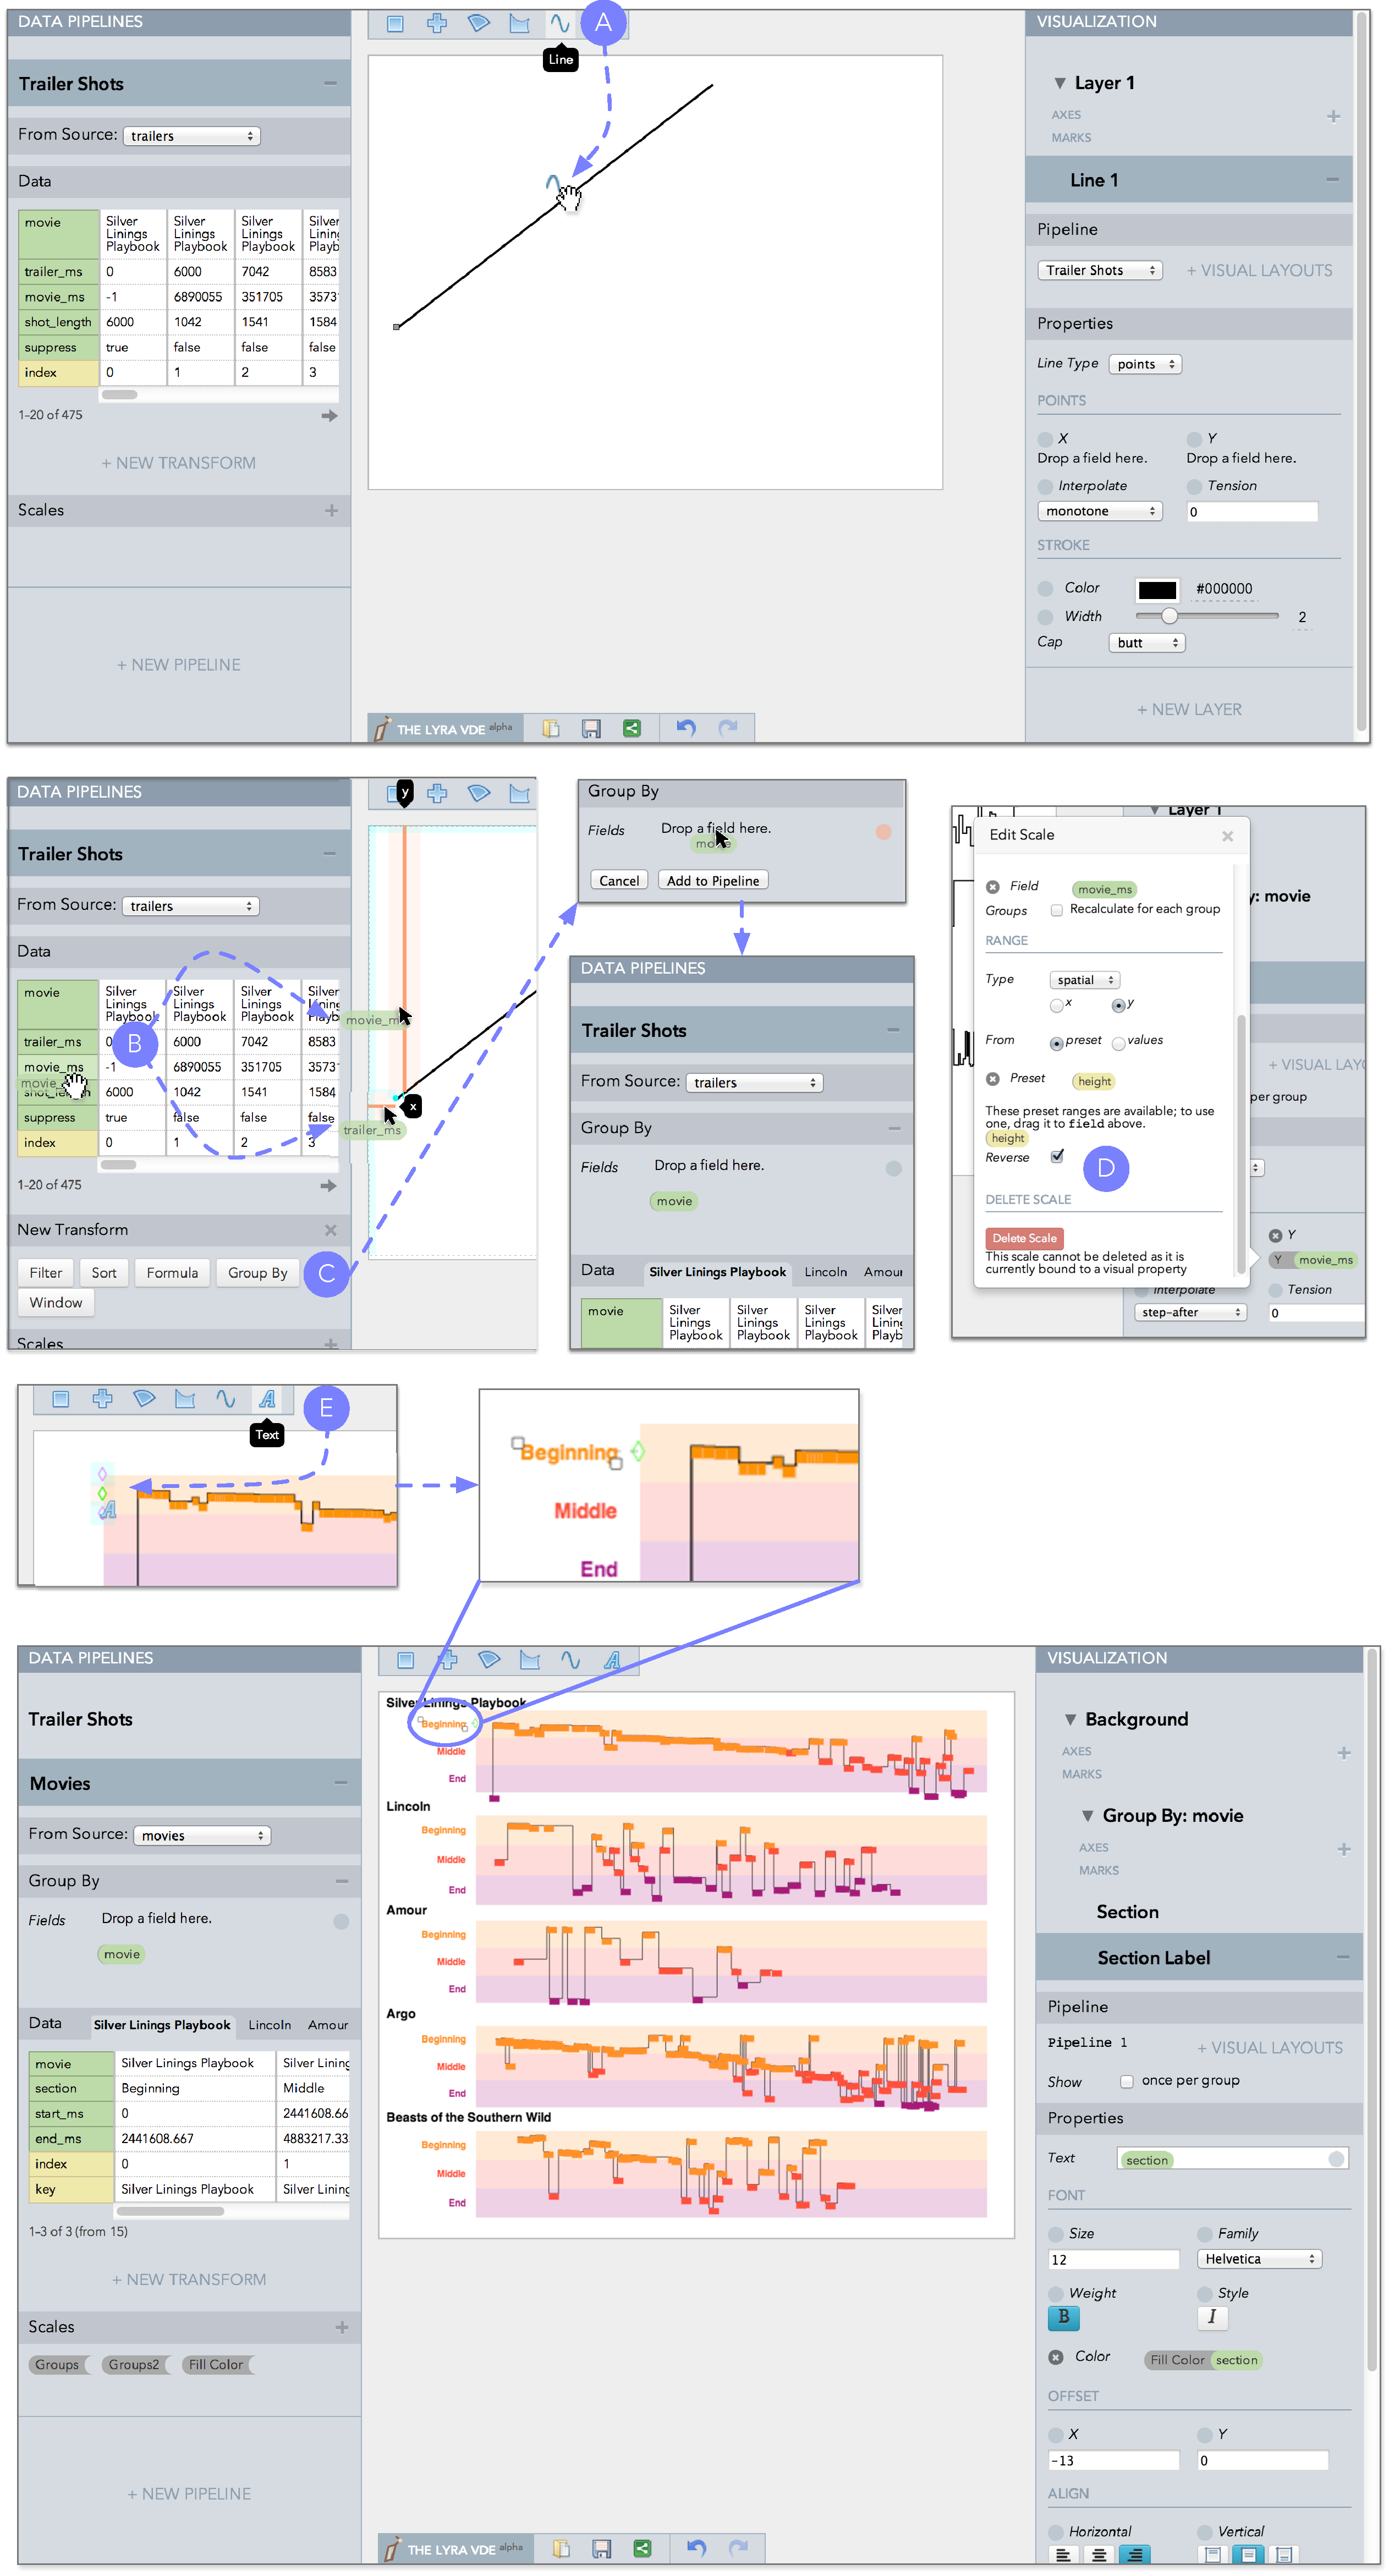
\includegraphics[width=0.7\textwidth]{usage}}
\end{figure}

We introduce lines by dragging a \emph{line mark} from the palette at the top of
the screen and dropping it on the canvas (Fig.~\ref{fig:lyra:usage}(a)). This
adds a new line (backed by a single datum) to the current layer and associates
it with a new data pipeline. The default pipeline is empty, as we have not yet
specified a data source. To register a new source, we provide a name and a URL
to our trailer shots data, and, upon load, review the inferred data types
(number, string, etc.) for each data field. The output of the pipeline is then
shown in the data table at the bottom of the pipeline inspector
(Fig.~\ref{fig:lyra:usage}(b)).

We bind data in the pipeline to visual properties of the line mark via
drag-and-drop of data fields. Dragging triggers the display of \emph{drop zones}
overlaid on the visualization canvas. Dropping a data field on a zone
establishes a visual encoding (Fig.~\ref{fig:lyra:usage}(b)). We drag
\texttt{trailer\_ms} and drop it over the line's \texttt{x} property, then drop
\texttt{movie\_ms} over \texttt{y}. These actions result in line segments
connecting every data point.

However, we desire separate line charts per film. To divide the data, we add a
\emph{group by} transformation to our pipeline (Fig.~\ref{fig:lyra:usage}(c)),
keyed on the movie title. The data table reflects the result via tabbed groups,
and the mark's property inspector now offers an option for group
\texttt{layout}. We choose a \texttt{vertical} layout to produce one line per
movie, arrayed down the canvas. We now see that the data includes shots that
appear in trailers but not in movies (identified by the \texttt{suppress}
field); we add a \emph{filter} transform to remove them
(Fig.~\ref{fig:lyra:usage}(d)). Next, we want film timelines oriented
top-to-bottom, but our lines show the reverse. We adjust the orientation of the
y-axis \emph{scale} by reversing its scale range (Fig.~\ref{fig:lyra:usage}(e)).

Next, we add small rectangle plots by dragging a \emph{rectangle mark} onto the
canvas. Lyra automatically associates the mark with the current pipeline and the
visualization now shows one rectangle per shot. As with the line mark, we drag
\texttt{trailer\_ms} and \texttt{movie\_ms} to the rectangle's \texttt{x} and
\texttt{y} property drop zones. We size the rectangles by dragging
\texttt{shot\_length} over the \texttt{width} drop zone and dragging the bottom
\emph{handle} to manually set the desired height (Fig.~\ref{fig:lyra:usage}(f)).
To color rectangles based on shot onset time in the film, we drag
\texttt{movie\_ms} over the \texttt{fill} property drop zone, and choose custom
colors in the resulting scale definition dialog.

The final step is to create labels and background rectangles to identify the
movies and their beginning, middle, and end sections. As these elements should
reside in the background, we create a new layer in Lyra. Movie section
information is drawn from a different data source, so we create a new pipeline.
We then drag a rectangle mark onto the canvas, and drag the section
\texttt{start} and \texttt{end} fields onto the rectangle \texttt{y} and
\texttt{y2} properties, resulting in a vertical layout for beginning, middle,
and end sections. We bind the \texttt{label} field to the fill color property
and select custom colors for the resulting scale mapping. To label each section,
we drag a \emph{text mark} from the palette and drop it on a rectangle's
diamond-shaped \emph{connector} (Fig.~\ref{fig:lyra:usage}(g)). Doing so anchors
the text mark coordinates to the rectangle. Finally, we bind the \texttt{label}
field as textual content and set the text fill color. We now can export the
visualization as either a Vega specification or an image file.
% !TEX root = ../thesis.tex
\vspace{-10pt}

\section{Example Visualizations}

\vspace{-10pt}

One of Lyra's primary goals is to enable an expressive design space. With Lyra,
it should be possible to create visualizations that would have previously
required programming. To assess the extent to which this goal has been met, we
constructed a diverse collection of example visualizations, including those
shown below. These examples compose multiple mark types, and many require
multiple data pipelines. For example, Fig.~\ref{fig:lyra:caltrain} uses line,
symbol, and text marks to convey two datasets: train routes and stations.
Fig.~\ref{fig:lyra:bertin} demonstrates that Lyra's integration of data
pipelines and graphical manipulation is necessary to maintain expressiveness:
shading the bars requires a data pipeline with \emph{Group By} and
\emph{Formula} data transformations applied.

Similarly, exposing visual layout inspectors allows for rapid design iteration.
In Fig.~\ref{fig:lyra:les_mis}, for example, the \emph{force-directed layout}
inspector exposes parameters such as link distance, strength and gravity;
adjusting them re-renders the layout in real-time. The layout also augments
direct manipulation on the canvas: designers can brush to select nodes and
double-click to pin them. Together, these facilitate a converging process:
pinning satisfactory nodes, adjusting layout properties, and re-running the
layout to reposition unpinned nodes. This process would be cumbersome using only
D3's force-directed layout~\cite{bostock:d3}: after programming the layout,
adjusting parameters requires editing the code and refreshing the browser.
Pinning nodes then requires inspecting the properties of each rendered node
individually and copying the \texttt{x} and \texttt{y} positions into the raw
dataset.

\begin{figure}[h!]
  \centering
  \includegraphics[width=\columnwidth]{bullet_chart}
  \caption{Bullet chart using rectangle and symbol marks grouped
by category. Labels are positioned via a left-edge connector on rectangles.}
  \label{fig:lyra:bulletChart}
\end{figure}

\begin{figure}[h!]
  \centering
  \includegraphics[width=\columnwidth]{driving}
  \caption{A recreation of \emph{Driving Shifts Into Reverse} by Hannah
  Fairfield from The New York Times, originally published May 2, 2010.}
  \label{fig:lyra:gas_driving}
\end{figure}

\begin{figure}[h!]
  \centering
  \includegraphics[width=\columnwidth]{les-mis}
  \caption{Character co-occurrences in Les
Mis\'{e}rables. Colors represent cluster memberships computed by a
community-detection algorithm.}
  \label{fig:lyra:les_mis}
\end{figure}

\begin{figure}[h!]
  \centering
  \includegraphics[width=\columnwidth]{caltrain}
  \caption{The schedule of the San Francisco Bay Area's CalTrain service in the style of E. J. Marey's Paris train schedule.}
  \label{fig:lyra:caltrain}
\end{figure}

\begin{figure}[h!]
  \centering
  \includegraphics[width=\columnwidth]{zipscribble}
  \caption{ZipScribble by Kosara~\cite{kosara:zipscribble}. A \emph{geo} layout
 encoder is used with line marks to connect latitude and longitudes of zip
 codes.}
  \label{fig:lyra:zipscribble}
\end{figure}

\begin{figure}[h!]
  \centering
  \includegraphics[width=\columnwidth]{streamgraph}
  \caption{A streamgraph of unemployed U.S. workers by industry, using a
  \emph{stack} layout with a \texttt{wiggle} offset~\cite{byron:streamgraph}.}
  \label{fig:lyra:streamgraph}
\end{figure}

\begin{figure}[h!]
  \centering
  \includegraphics[width=\columnwidth]{napoleon}
  \caption{Minard's map of Napoleon's Russian campaign. A \emph{geo} transform
 encodes spatial positions; army size maps to line stroke width.}
  \label{fig:lyra:napoleon}
\end{figure}

\begin{figure}[h!]
  \centering
  \includegraphics[width=\columnwidth]{bertin}
  \caption{Jacques Bertin's analysis of hotel patterns. \emph{Group by} and \emph{formula}
 transforms are used to shade bars with values above the mean.}
  \label{fig:lyra:bertin}
\end{figure}

\clearpage

\subsection{Limitations}

\vspace{-7pt}

\Cref{fig:lyra:usage,fig:lyra:bulletChart,fig:lyra:gas_driving,fig:lyra:les_mis,fig:lyra:caltrain,fig:lyra:zipscribble,fig:lyra:streamgraph,fig:lyra:napoleon,fig:lyra:bertin}
demonstrate that Lyra enables an expressive design space, but creating these
examples also reveals some limitations. Vega currently lacks support for polar
coordinates. As a result, Lyra cannot (yet) provide \emph{arc} mark connectors
or produce radial axes, making it difficult to recreate classic visualizations
such as Nightingale's Rose or Burtin's antibiotics chart. Additionally, Lyra
only supports the \textsc{rgb} color space, while Vega also supports
\textsc{hsl}, \textsc{lab}, and \textsc{hcl}. These color spaces facilitate
perceptually-sound designs. We plan to address these limitations in future
versions of Vega and Lyra.
% !TEX root = ../thesis.tex

\vspace{-10pt}

\section{Formative User Evaluations}

\vspace{-10pt}

Lyra was designed to support both expressive and \emph{accessible} visualization
design: users should not require coding expertise to be able to construct custom
visualizations. To evaluate Lyra's accessibility, we conducted first-use studies
with 15 representative users including 6 data analysts / visualization
designers, 5 data journalists, and 4 graduate students in data visualization. On
10-point scales, the median self-reported visualization design expertise was 7,
while programming expertise range between 2--8. These users all use
visualization as a communicative medium but their processes for creating them
vary. The visualization designers and grad students were more technically
proficient and typically use D3, whereas the data journalists rely on chart
typologies (Microsoft Excel) or grammar-based systems (Tableau) that do not
require programming. Some journalists also reported eschewing visualization
systems in favor of drawing programs such as Adobe Illustrator.

\vspace{-10pt}

\subsection{Methods}

\vspace{-7pt}

We began each study with a 10 minute tutorial. We then asked participants to
design three graphics: a bar chart of medal count by country at the 2012
Olympics (T1), a grouped or stacked bar chart of medal counts by medal type and
country (T2), and a trellis plot of barley yields (T3,
Fig.~\ref{fig:lyra:trellis}). These tasks were designed to ensure participants
interacted with all aspects of Lyra. Each task was more difficult than the
previous, intending to first familiarize participants with the Lyra design
process, and then challenge them. Participants were encouraged to think-aloud
and were de-briefed at the end. Sessions lasted approximately 45 minutes, after
which we administered a post-study survey.

\begin{figure}[b!]
  \centering
  \includegraphics[width=1\columnwidth]{barley}
  \caption{Study participants recreated the barley yields Trellis
  display~\cite{becker:trellis}.}
  \label{fig:lyra:trellis}
\end{figure}

\vspace{-10pt}

\subsection{Successes}

\vspace{-7pt}

Users quickly learned Lyra's interaction model and all users, regardless of
their technical expertise, successfully completed all three tasks with minimal
guidance (100\% task completion rate). Users completed the first two tasks in
just a few minutes, the more complex third task took longer (T1: median time =
1:33, inter-quartile range (IQR) = 0:51; T2: median = 2:43, IQR = 2:57; T3:
median = 10:24, IQR = 4:00). In a post- study survey, users rated Lyra's
interface highly: drop zones felt natural to use ($\mu$ = 4.4, $\sigma$ = 0.57
on a 5-point Likert scale), connectors helped to relatively position marks
($\mu$ = 4.3, $\sigma$ = 0.49), and a pipeline's data table helped evaluate
context ($\mu$ = 4.4, $\sigma$ = 0.51). Handles were found useful for resizing
and positioning ($\mu$ = 3.8, $\sigma$ = 0.45) but users noted that the
properties they control are typically mapped to data. When asked to recount
their experience, users described drop zones as \emph{``natural''} and
\emph{``intuitive.''} One user stated, ``\emph{it's like \emph{literally} saying
`put that there.'}'' Others drew comparisons to Tableau's shelves:
\emph{``[shelves] don't always behave like I expect them to but [drop zones]
make me feel more in control.''} One participant ended his session by saying
that \emph{``there's a real joy in using Lyra.''}

Two journalists who participated lead data visualization teams in their
organizations. They appreciated that Lyra took cues from familiar drawing tools.
They welcomed Lyra's image export options, particularly SVG export, as the
visualizations they produce are often reutilized in print media. One suggested
that Lyra could be a powerful training tool that could help familiarize his team
with the process of designing visualizations from the ground-up.

\begin{figure}[b!]
\centering
  \includegraphics[width=\columnwidth]{sara}
  \caption{A study participant approximately recreated a D3 visualization (left,
  requiring 4-6 hours) in Lyra (right, requiring only 10 minutes).}
  \label{fig:lyra:sara_waitlists}
\end{figure}

Users familiar with lower-level tools such as D3 found Lyra useful for rapidly
prototyping and iterating on their design. For example, one user (self-rated
expertise with D3 as 6.5/10) used Lyra with her own data. By her estimate, she
had previously spent between 4--6 hours repurposing an existing D3 example to
create a custom visualization. She was able to create a close approximation in
Lyra, shown in \cref{fig:lyra:sara_waitlists}, in only 10 minutes.

\subsection{Shortcomings}

We also observed that Lyra posed certain challenges for our participants.
Although users found drop zones natural and intuitive, they noted problems with
the current implementation. First, when users missed a drop zone by a few
pixels, they expected Lyra to infer their intent. Second, when users
successfully dropped a field, they would lose track of the currently selected
mark if it was repositioned. A third shortcoming was Lyra's lack of support for
undo, which led users to become more hesitant to freely explore. Undo support
has since been added to Lyra, and we plan to address the remaining issues in
future versions. For example, a Voronoi diagram could be used to find the
nearest drop zone~\cite{grossman:bubble}, and staggered animated transitions
could help users better track changes~\cite{heer:animated} to marks.

Finally, several users mentioned that learning from and repurposing existing
visualizations is an important part of their design process. They found the
blank canvas to be an intimidating starting point. We anticipate that
providing a gallery of examples (including those in this paper) that users can
import, reuse and modify would mitigate this issue.

% !TEX root = ../thesis.tex
\vspace{-10pt}

\section{Reflections \& Future Work}

\vspace{-10pt}

\begin{figure}[b!]
\includegraphics[width=\columnwidth]{lyra2}
\caption{The new Lyra interface. The side panels from \cref{fig:lyra:inspectors}
have been redesigned and consolidated to the left-hand side. As the user drags a
data field across the canvas, the nearest drop zone (highlighted in orange) is
automatically selected\,---\,a technique known as a bubble
cursor~\cite{grossman:bubble}.}
\label{fig:lyra2}
\end{figure}

Chronologically, Lyra was the first project to form part of this dissertation.
At the time of writing, a new version, that leverages Reactive Vega and
Vega-Lite, is under development. Thus, it is worth reflecting on how its role in
the ecosystem has evolved.

Much of Lyra's existing functionality can now be driven purely via a Reactive
Vega specification rather than through external callbacks. For instance, direct
manipulation operations on handles are now driven entirely via signals, rather
than event handling callbacks. Similarly, connectors make use of reactive
geometry directly. A bubble cursor~\cite{grossman:bubble} UDF (see
\cref{sec:udfs}) is registered to accelerate drop zone selection, as shown in
\cref{fig:lyra2}, addressing a major shortcoming users identified previously.

Moreover, Lyra's built-in production rule system has been subsumed by Vega-Lite.
Now, when users drag a data field onto a drop zone, a Vega-Lite unit
specification is compiled, the resultant Vega specification is statically
analyzed, and components selectively merged or updated in Lyra's backing Vega
specification.

With these changes, Lyra's place in the tool stack comes into sharper relief: it
\emph{bridges} two levels of abstraction within a single, cohesive environment.
Direct manipulation operations occur at the Vega-Lite level, and allow users to
rapidly generate recognizable visualizations. For more fine-grained
manipulation, or for custom design elements, users drop down to the Vega level
by interacting with the visual inspectors. A critical advantage of this approach
is that users can fluidly work with the level of abstraction best suited for the
task at hand. In fact, they may be altogether unaware of the separate roles
played by Vega and Vega-Lite under-the-hood!

Looking ahead, an exciting challenge is how Lyra might be extended to support
the design of \emph{interactive} visualizations. In-keeping with the above
approach, perhaps direct manipulation interactions (or demonstrations) should
generate Vega-Lite selections, which can be further modified with signal and
predicate inspectors.

Similarly, while Lyra's primary focus is currently on design tasks, data
visualization inevitably requires data cleaning and transformation. Lyra's data
pipelines offer sufficient flexibility to support analytic tasks, but require
familiarity with transformation operators. Can direct manipulation methods, akin
to those in Data Wrangler~\cite{kandel:wrangler}, be further incorporated to
specify more complex data transformations?
% !TEX root = ../thesis.tex

\vspace{-20pt}

\section{Conclusion \& Future Work}
\label{sec:vg:conclusion}

\vspace{-10pt}

Declarative languages are a popular means of authoring
visualizations~\cite{bostock:protovis, bostock:d3, heer:protovisjava}, but have
lacked first-class support for interaction design. In response, we contribute
Reactive Vega, the first language and system architecture to support declarative
visualization and interaction design in a comprehensive and performant fashion.

It is important to note that although Reactive Vega provides an complete
end\--to\--end system\,---\,whereby users invoke the parser to traverse an input
declarative specification and instantiate the necessary architecture components
to render a visualization\,---\,this process can be decoupled. Reactive Vega's
declarative model can be implemented as extensions to D3, and higher-level tools
can manually construct and connect dataflow operators.

By facilitating programmatic generation of visualization, Reactive Vega's
declarative \textsc{json} syntax has led to a growing ecosystem of higher-level
visualization systems. For example, MapD~\cite{mapd:vega} has integrated Vega
with their \textsc{gpu}-powered database; custom \textsc{sql} queries can be
embedded within the \textsc{json} specification, which are dispatched to the
backend server, rendered, and returned to the client as a \textsc{png} image.
Similarly, Wikipedia, a security-concious environment where it would be
difficult to allow users to write imperative visualization code, has integrated
Vega~\cite{mediawiki:graph} to embed interactive visualizations within articles.

Still, improved support for authoring and debugging Vega specifications remains
a promising avenue for future work. For instance, Hoffswell
et~al.~\cite{hoffswell:debugging} developed a ``time-traveling'' debugger for
Reactive Vega specifications and found that first-time Vega users were able to
accurately trace errors through the specification. Further work, particularly by
instrumenting Reactive Vega's dataflow graph to enable inspection and stepping
through changeset propagation could aid in learnability~\cite{guo:tutor}.
Through the development of such tools, we can also assess the accessibility of
the language. Can new users learn the declarative interaction model? Can
experts, accustomed to callback-driven programming, adapt quickly?

Reactive Vega's architecture also offers opportunities to study scalable
visualization design. Interactive visualization of large-scale datasets often
requires offloading computation to server-side architectures. For example,
Nanocubes~\cite{lins:nanocubes} and imMens~\cite{liu:immens} assemble
multi\--dimensional data cubes that can be decomposed into smaller data tiles
and pushed to the client. Such components could be integrated into a dataflow
graph with execution distributed across server and client~\cite{domoritz:dsia}.
For example, as the dataflow graph scheduler is responsible for propagation, it
might anticipate possible user interactions and prefetch data tiles in order to
reduce latency~\cite{battle:prefetch}.

Reactive Vega is an open source system available at
\url{http://vega.github.io/vega/}.

\bibliographystyle{abbrv}
\bibliography{thesis}
\end{document}